\documentclass[twoside]{book}

% Packages required by doxygen
\usepackage{fixltx2e}
\usepackage{calc}
\usepackage{doxygen}
\usepackage[export]{adjustbox} % also loads graphicx
\usepackage{graphicx}
\usepackage[utf8]{inputenc}
\usepackage{makeidx}
\usepackage{multicol}
\usepackage{multirow}
\PassOptionsToPackage{warn}{textcomp}
\usepackage{textcomp}
\usepackage[nointegrals]{wasysym}
\usepackage[table]{xcolor}

% Font selection
\usepackage[T1]{fontenc}
\usepackage[scaled=.90]{helvet}
\usepackage{courier}
\usepackage{amssymb}
\usepackage{sectsty}
\renewcommand{\familydefault}{\sfdefault}
\allsectionsfont{%
  \fontseries{bc}\selectfont%
  \color{darkgray}%
}
\renewcommand{\DoxyLabelFont}{%
  \fontseries{bc}\selectfont%
  \color{darkgray}%
}
\newcommand{\+}{\discretionary{\mbox{\scriptsize$\hookleftarrow$}}{}{}}

% Page & text layout
\usepackage{geometry}
\geometry{%
  a4paper,%
  top=2.5cm,%
  bottom=2.5cm,%
  left=2.5cm,%
  right=2.5cm%
}
\tolerance=750
\hfuzz=15pt
\hbadness=750
\setlength{\emergencystretch}{15pt}
\setlength{\parindent}{0cm}
\setlength{\parskip}{3ex plus 2ex minus 2ex}
\makeatletter
\renewcommand{\paragraph}{%
  \@startsection{paragraph}{4}{0ex}{-1.0ex}{1.0ex}{%
    \normalfont\normalsize\bfseries\SS@parafont%
  }%
}
\renewcommand{\subparagraph}{%
  \@startsection{subparagraph}{5}{0ex}{-1.0ex}{1.0ex}{%
    \normalfont\normalsize\bfseries\SS@subparafont%
  }%
}
\makeatother

% Headers & footers
\usepackage{fancyhdr}
\pagestyle{fancyplain}
\fancyhead[LE]{\fancyplain{}{\bfseries\thepage}}
\fancyhead[CE]{\fancyplain{}{}}
\fancyhead[RE]{\fancyplain{}{\bfseries\leftmark}}
\fancyhead[LO]{\fancyplain{}{\bfseries\rightmark}}
\fancyhead[CO]{\fancyplain{}{}}
\fancyhead[RO]{\fancyplain{}{\bfseries\thepage}}
\fancyfoot[LE]{\fancyplain{}{}}
\fancyfoot[CE]{\fancyplain{}{}}
\fancyfoot[RE]{\fancyplain{}{\bfseries\scriptsize Generated by Doxygen }}
\fancyfoot[LO]{\fancyplain{}{\bfseries\scriptsize Generated by Doxygen }}
\fancyfoot[CO]{\fancyplain{}{}}
\fancyfoot[RO]{\fancyplain{}{}}
\renewcommand{\footrulewidth}{0.4pt}
\renewcommand{\chaptermark}[1]{%
  \markboth{#1}{}%
}
\renewcommand{\sectionmark}[1]{%
  \markright{\thesection\ #1}%
}

% Indices & bibliography
\usepackage{natbib}
\usepackage[titles]{tocloft}
\setcounter{tocdepth}{3}
\setcounter{secnumdepth}{5}
\makeindex

% Hyperlinks (required, but should be loaded last)
\usepackage{ifpdf}
\ifpdf
  \usepackage[pdftex,pagebackref=true]{hyperref}
\else
  \usepackage[ps2pdf,pagebackref=true]{hyperref}
\fi
\hypersetup{%
  colorlinks=true,%
  linkcolor=blue,%
  citecolor=blue,%
  unicode%
}

% Custom commands
\newcommand{\clearemptydoublepage}{%
  \newpage{\pagestyle{empty}\cleardoublepage}%
}

\usepackage{caption}
\captionsetup{labelsep=space,justification=centering,font={bf},singlelinecheck=off,skip=4pt,position=top}

%===== C O N T E N T S =====

\begin{document}

% Titlepage & ToC
\hypersetup{pageanchor=false,
             bookmarksnumbered=true,
             pdfencoding=unicode
            }
\pagenumbering{alph}
\begin{titlepage}
\vspace*{7cm}
\begin{center}%
{\Large My Project \\[1ex]\large 1.\+0 }\\
\vspace*{1cm}
{\large Generated by Doxygen 1.8.14}\\
\end{center}
\end{titlepage}
\clearemptydoublepage
\pagenumbering{roman}
\tableofcontents
\clearemptydoublepage
\pagenumbering{arabic}
\hypersetup{pageanchor=true}

%--- Begin generated contents ---
\chapter{Namespace Index}
\section{Namespace List}
Here is a list of all documented namespaces with brief descriptions\+:\begin{DoxyCompactList}
\item\contentsline{section}{\mbox{\hyperlink{namespace_poke_quet}{Poke\+Quet}} }{\pageref{namespace_poke_quet}}{}
\end{DoxyCompactList}

\chapter{Hierarchical Index}
\section{Class Hierarchy}
This inheritance list is sorted roughly, but not completely, alphabetically\+:\begin{DoxyCompactList}
\item \contentsline{section}{Poke\+Quet.\+Card}{\pageref{class_poke_quet_1_1_card}}{}
\item Dialog\begin{DoxyCompactList}
\item \contentsline{section}{Poke\+Quet.\+Game\+Over\+Dialog}{\pageref{class_poke_quet_1_1_game_over_dialog}}{}
\end{DoxyCompactList}
\item List\begin{DoxyCompactList}
\item \contentsline{section}{Poke\+Quet.\+Deck}{\pageref{class_poke_quet_1_1_deck}}{}
\end{DoxyCompactList}
\item \contentsline{section}{Poke\+Quet.\+Main\+Class}{\pageref{class_poke_quet_1_1_main_class}}{}
\item \contentsline{section}{Poke\+Quet.\+Player}{\pageref{class_poke_quet_1_1_player}}{}
\begin{DoxyCompactList}
\item \contentsline{section}{Poke\+Quet.\+A\+I\+Player}{\pageref{class_poke_quet_1_1_a_i_player}}{}
\begin{DoxyCompactList}
\item \contentsline{section}{Poke\+Quet.\+A\+I\+Player\+Random}{\pageref{class_poke_quet_1_1_a_i_player_random}}{}
\item \contentsline{section}{Poke\+Quet.\+A\+I\+Player\+Simple}{\pageref{class_poke_quet_1_1_a_i_player_simple}}{}
\end{DoxyCompactList}
\end{DoxyCompactList}
\item Window\begin{DoxyCompactList}
\item \contentsline{section}{Main\+Window}{\pageref{class_main_window}}{}
\item \contentsline{section}{Poke\+Quet.\+Main\+Menu}{\pageref{class_poke_quet_1_1_main_menu}}{}
\end{DoxyCompactList}
\end{DoxyCompactList}

\chapter{Class Index}
\section{Class List}
Here are the classes, structs, unions and interfaces with brief descriptions\+:\begin{DoxyCompactList}
\item\contentsline{section}{\mbox{\hyperlink{class_poke_quet_1_1_a_i_player}{Poke\+Quet.\+A\+I\+Player}} \\*Eine Klasse für Computergesteuerte Gegner die selbstständig Züge machen. }{\pageref{class_poke_quet_1_1_a_i_player}}{}
\item\contentsline{section}{\mbox{\hyperlink{class_poke_quet_1_1_a_i_player_random}{Poke\+Quet.\+A\+I\+Player\+Random}} \\*KI für leichten Computergegner, der völlig zufällige Disziplinen auswählt. }{\pageref{class_poke_quet_1_1_a_i_player_random}}{}
\item\contentsline{section}{\mbox{\hyperlink{class_poke_quet_1_1_a_i_player_simple}{Poke\+Quet.\+A\+I\+Player\+Simple}} \\*KI für schweren Computergegner, der logische Entscheidungen trifft und immer den höchsten Wert wählt, aber Type ignoriert. }{\pageref{class_poke_quet_1_1_a_i_player_simple}}{}
\item\contentsline{section}{\mbox{\hyperlink{class_poke_quet_1_1_card}{Poke\+Quet.\+Card}} \\*Klasse die eine Karte darstellt und durch Modelbinding via J\+S\+O\+N.\+N\+ET zusammengebaut wird. }{\pageref{class_poke_quet_1_1_card}}{}
\item\contentsline{section}{\mbox{\hyperlink{class_poke_quet_1_1_deck}{Poke\+Quet.\+Deck}} \\*Klasse die ein Kartendeck darstellt und keine }{\pageref{class_poke_quet_1_1_deck}}{}
\item\contentsline{section}{\mbox{\hyperlink{class_poke_quet_1_1_game_over_dialog}{Poke\+Quet.\+Game\+Over\+Dialog}} \\*Fenster das nach Ende des Spiels erscheint und den Sieger bzw. Unentschieden anzeigt und die Option für Neustart oder Ende des aktuellen Spiels gibt }{\pageref{class_poke_quet_1_1_game_over_dialog}}{}
\item\contentsline{section}{\mbox{\hyperlink{class_poke_quet_1_1_main_class}{Poke\+Quet.\+Main\+Class}} }{\pageref{class_poke_quet_1_1_main_class}}{}
\item\contentsline{section}{\mbox{\hyperlink{class_poke_quet_1_1_main_menu}{Poke\+Quet.\+Main\+Menu}} }{\pageref{class_poke_quet_1_1_main_menu}}{}
\item\contentsline{section}{\mbox{\hyperlink{class_main_window}{Main\+Window}} \\*Das Hauptfenster (das Spiel) }{\pageref{class_main_window}}{}
\item\contentsline{section}{\mbox{\hyperlink{class_poke_quet_1_1_player}{Poke\+Quet.\+Player}} }{\pageref{class_poke_quet_1_1_player}}{}
\end{DoxyCompactList}

\chapter{Namespace Documentation}
\hypertarget{namespace_poke_quet}{}\section{Poke\+Quet Namespace Reference}
\label{namespace_poke_quet}\index{Poke\+Quet@{Poke\+Quet}}
\subsection*{Classes}
\begin{DoxyCompactItemize}
\item 
class \mbox{\hyperlink{class_poke_quet_1_1_a_i_player}{A\+I\+Player}}
\begin{DoxyCompactList}\small\item\em Eine Klasse für Computergesteuerte Gegner die selbstständig Züge machen. \end{DoxyCompactList}\item 
class \mbox{\hyperlink{class_poke_quet_1_1_a_i_player_random}{A\+I\+Player\+Random}}
\begin{DoxyCompactList}\small\item\em KI für leichten Computergegner, der völlig zufällige Disziplinen auswählt. \end{DoxyCompactList}\item 
class \mbox{\hyperlink{class_poke_quet_1_1_a_i_player_simple}{A\+I\+Player\+Simple}}
\begin{DoxyCompactList}\small\item\em KI für schweren Computergegner, der logische Entscheidungen trifft und immer den höchsten Wert wählt, aber Type ignoriert. \end{DoxyCompactList}\item 
class \mbox{\hyperlink{class_poke_quet_1_1_card}{Card}}
\begin{DoxyCompactList}\small\item\em Klasse die eine Karte darstellt und durch Modelbinding via J\+S\+O\+N.\+N\+ET zusammengebaut wird. \end{DoxyCompactList}\item 
class \mbox{\hyperlink{class_poke_quet_1_1_deck}{Deck}}
\begin{DoxyCompactList}\small\item\em Klasse die ein Kartendeck darstellt und keine \end{DoxyCompactList}\item 
class \mbox{\hyperlink{class_poke_quet_1_1_game_over_dialog}{Game\+Over\+Dialog}}
\begin{DoxyCompactList}\small\item\em Fenster das nach Ende des Spiels erscheint und den Sieger bzw. Unentschieden anzeigt und die Option für Neustart oder Ende des aktuellen Spiels gibt \end{DoxyCompactList}\item 
class \mbox{\hyperlink{class_poke_quet_1_1_main_class}{Main\+Class}}
\item 
class \mbox{\hyperlink{class_poke_quet_1_1_main_menu}{Main\+Menu}}
\item 
class \mbox{\hyperlink{class_poke_quet_1_1_player}{Player}}
\end{DoxyCompactItemize}
\subsection*{Enumerations}
\begin{DoxyCompactItemize}
\item 
enum \mbox{\hyperlink{namespace_poke_quet_aa425f1b8cf90847021fe1177d6a7199d}{Discipline}} \{ \newline
{\bfseries T\+Y\+PE}, 
{\bfseries HP}, 
{\bfseries A\+TK}, 
{\bfseries D\+EF}, 
\newline
{\bfseries S\+PD}
 \}
\begin{DoxyCompactList}\small\item\em Ein Enum der die Kartendisziplinen darstellt. \end{DoxyCompactList}\end{DoxyCompactItemize}


\subsection{Enumeration Type Documentation}
\mbox{\Hypertarget{namespace_poke_quet_aa425f1b8cf90847021fe1177d6a7199d}\label{namespace_poke_quet_aa425f1b8cf90847021fe1177d6a7199d}} 
\index{Poke\+Quet@{Poke\+Quet}!Discipline@{Discipline}}
\index{Discipline@{Discipline}!Poke\+Quet@{Poke\+Quet}}
\subsubsection{\texorpdfstring{Discipline}{Discipline}}
{\footnotesize\ttfamily enum \mbox{\hyperlink{namespace_poke_quet_aa425f1b8cf90847021fe1177d6a7199d}{Poke\+Quet.\+Discipline}}\hspace{0.3cm}{\ttfamily [strong]}}



Ein Enum der die Kartendisziplinen darstellt. 


\chapter{Class Documentation}
\hypertarget{class_poke_quet_1_1_a_i_player}{}\section{Poke\+Quet.\+A\+I\+Player Class Reference}
\label{class_poke_quet_1_1_a_i_player}\index{Poke\+Quet.\+A\+I\+Player@{Poke\+Quet.\+A\+I\+Player}}


Eine Klasse für Computergesteuerte Gegner die selbstständig Züge machen.  


Inheritance diagram for Poke\+Quet.\+A\+I\+Player\+:\begin{figure}[H]
\begin{center}
\leavevmode
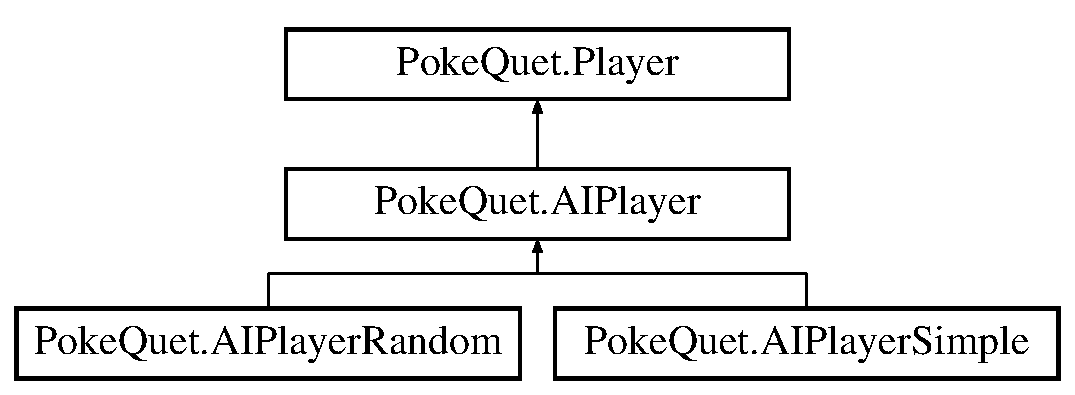
\includegraphics[height=3.000000cm]{class_poke_quet_1_1_a_i_player}
\end{center}
\end{figure}
\subsection*{Public Member Functions}
\begin{DoxyCompactItemize}
\item 
\mbox{\Hypertarget{class_poke_quet_1_1_a_i_player_aa003be7c23e044540792bfb254b58b45}\label{class_poke_quet_1_1_a_i_player_aa003be7c23e044540792bfb254b58b45}} 
{\bfseries A\+I\+Player} (string name)
\item 
void \mbox{\hyperlink{class_poke_quet_1_1_a_i_player_a91da43db7587617dbfe7858a6fafd434}{Init}} (\mbox{\hyperlink{class_poke_quet_1_1_card}{Card}}\mbox{[}$\,$\mbox{]} card\+Pool)
\begin{DoxyCompactList}\small\item\em Eine Methode zum initialisieren der KI sodass diese aufgrund des Kartensatzes z.\+B. die statitisch optimale Disziplin für jede Karte berechnen könnten, aber das Umzusetzen erfordert den ganzen Disziplinvergleich selbst zu implementieren oder das der Disziplinvergleich vom restlichen Spielverlauf getrennt wird. \end{DoxyCompactList}\item 
abstract \mbox{\hyperlink{namespace_poke_quet_aa425f1b8cf90847021fe1177d6a7199d}{Discipline}} \mbox{\hyperlink{class_poke_quet_1_1_a_i_player_ae2862ead657c524614793ea4d3ebf80b}{Make\+Turn}} (\mbox{\hyperlink{class_poke_quet_1_1_player}{Player}} opponent, \mbox{\hyperlink{class_poke_quet_1_1_deck}{Deck}} tie\+Cards)
\begin{DoxyCompactList}\small\item\em Die Methode zur Bestimmung des Zugs des Computerspielers \end{DoxyCompactList}\end{DoxyCompactItemize}
\subsection*{Static Public Attributes}
\begin{DoxyCompactItemize}
\item 
static readonly \mbox{\hyperlink{namespace_poke_quet_aa425f1b8cf90847021fe1177d6a7199d}{Discipline}} \mbox{[}$\,$\mbox{]} \mbox{\hyperlink{class_poke_quet_1_1_a_i_player_a72ab201b6fd3e18713da18d17824179a}{D\+I\+S\+C\+I\+P\+L\+I\+N\+ES}} = (\mbox{\hyperlink{namespace_poke_quet_aa425f1b8cf90847021fe1177d6a7199d}{Discipline}}\mbox{[}$\,$\mbox{]})Enum.\+Get\+Values(typeof(\mbox{\hyperlink{namespace_poke_quet_aa425f1b8cf90847021fe1177d6a7199d}{Discipline}}))
\begin{DoxyCompactList}\small\item\em Ein Array aller Disziplinen in \mbox{\hyperlink{namespace_poke_quet_aa425f1b8cf90847021fe1177d6a7199d}{Discipline}} \end{DoxyCompactList}\end{DoxyCompactItemize}
\subsection*{Additional Inherited Members}


\subsection{Detailed Description}
Eine Klasse für Computergesteuerte Gegner die selbstständig Züge machen. 



\subsection{Member Function Documentation}
\mbox{\Hypertarget{class_poke_quet_1_1_a_i_player_a91da43db7587617dbfe7858a6fafd434}\label{class_poke_quet_1_1_a_i_player_a91da43db7587617dbfe7858a6fafd434}} 
\index{Poke\+Quet\+::\+A\+I\+Player@{Poke\+Quet\+::\+A\+I\+Player}!Init@{Init}}
\index{Init@{Init}!Poke\+Quet\+::\+A\+I\+Player@{Poke\+Quet\+::\+A\+I\+Player}}
\subsubsection{\texorpdfstring{Init()}{Init()}}
{\footnotesize\ttfamily void Poke\+Quet.\+A\+I\+Player.\+Init (\begin{DoxyParamCaption}\item[{\mbox{\hyperlink{class_poke_quet_1_1_card}{Card}} \mbox{[}$\,$\mbox{]}}]{card\+Pool }\end{DoxyParamCaption})\hspace{0.3cm}{\ttfamily [inline]}}



Eine Methode zum initialisieren der KI sodass diese aufgrund des Kartensatzes z.\+B. die statitisch optimale Disziplin für jede Karte berechnen könnten, aber das Umzusetzen erfordert den ganzen Disziplinvergleich selbst zu implementieren oder das der Disziplinvergleich vom restlichen Spielverlauf getrennt wird. 


\begin{DoxyParams}{Parameters}
{\em card\+Pool} & Der komplette Kartensatz\\
\hline
\end{DoxyParams}


Diese Methode ist obsolet\mbox{\Hypertarget{class_poke_quet_1_1_a_i_player_ae2862ead657c524614793ea4d3ebf80b}\label{class_poke_quet_1_1_a_i_player_ae2862ead657c524614793ea4d3ebf80b}} 
\index{Poke\+Quet\+::\+A\+I\+Player@{Poke\+Quet\+::\+A\+I\+Player}!Make\+Turn@{Make\+Turn}}
\index{Make\+Turn@{Make\+Turn}!Poke\+Quet\+::\+A\+I\+Player@{Poke\+Quet\+::\+A\+I\+Player}}
\subsubsection{\texorpdfstring{Make\+Turn()}{MakeTurn()}}
{\footnotesize\ttfamily abstract \mbox{\hyperlink{namespace_poke_quet_aa425f1b8cf90847021fe1177d6a7199d}{Discipline}} Poke\+Quet.\+A\+I\+Player.\+Make\+Turn (\begin{DoxyParamCaption}\item[{\mbox{\hyperlink{class_poke_quet_1_1_player}{Player}}}]{opponent,  }\item[{\mbox{\hyperlink{class_poke_quet_1_1_deck}{Deck}}}]{tie\+Cards }\end{DoxyParamCaption})\hspace{0.3cm}{\ttfamily [pure virtual]}}



Die Methode zur Bestimmung des Zugs des Computerspielers 


\begin{DoxyParams}{Parameters}
{\em opponent} & Der gegnerische Spieler\\
\hline
{\em tie\+Cards} & Der Stich-\/\+Stapel\\
\hline
\end{DoxyParams}
\begin{DoxyReturn}{Returns}
Die Disziplin die als Zug gewählt wird.
\end{DoxyReturn}


Implemented in \mbox{\hyperlink{class_poke_quet_1_1_a_i_player_simple_a4c48360666f3fc8b7400cbfa2c7ea29e}{Poke\+Quet.\+A\+I\+Player\+Simple}}, and \mbox{\hyperlink{class_poke_quet_1_1_a_i_player_random_a8723ee791e3ac1ea34033cd6ce49398f}{Poke\+Quet.\+A\+I\+Player\+Random}}.



\subsection{Member Data Documentation}
\mbox{\Hypertarget{class_poke_quet_1_1_a_i_player_a72ab201b6fd3e18713da18d17824179a}\label{class_poke_quet_1_1_a_i_player_a72ab201b6fd3e18713da18d17824179a}} 
\index{Poke\+Quet\+::\+A\+I\+Player@{Poke\+Quet\+::\+A\+I\+Player}!D\+I\+S\+C\+I\+P\+L\+I\+N\+ES@{D\+I\+S\+C\+I\+P\+L\+I\+N\+ES}}
\index{D\+I\+S\+C\+I\+P\+L\+I\+N\+ES@{D\+I\+S\+C\+I\+P\+L\+I\+N\+ES}!Poke\+Quet\+::\+A\+I\+Player@{Poke\+Quet\+::\+A\+I\+Player}}
\subsubsection{\texorpdfstring{D\+I\+S\+C\+I\+P\+L\+I\+N\+ES}{DISCIPLINES}}
{\footnotesize\ttfamily readonly \mbox{\hyperlink{namespace_poke_quet_aa425f1b8cf90847021fe1177d6a7199d}{Discipline}} \mbox{[}$\,$\mbox{]} Poke\+Quet.\+A\+I\+Player.\+D\+I\+S\+C\+I\+P\+L\+I\+N\+ES = (\mbox{\hyperlink{namespace_poke_quet_aa425f1b8cf90847021fe1177d6a7199d}{Discipline}}\mbox{[}$\,$\mbox{]})Enum.\+Get\+Values(typeof(\mbox{\hyperlink{namespace_poke_quet_aa425f1b8cf90847021fe1177d6a7199d}{Discipline}}))\hspace{0.3cm}{\ttfamily [static]}}



Ein Array aller Disziplinen in \mbox{\hyperlink{namespace_poke_quet_aa425f1b8cf90847021fe1177d6a7199d}{Discipline}} 



The documentation for this class was generated from the following file\+:\begin{DoxyCompactItemize}
\item 
Player.\+cs\end{DoxyCompactItemize}

\hypertarget{class_poke_quet_1_1_a_i_player_random}{}\section{Poke\+Quet.\+A\+I\+Player\+Random Class Reference}
\label{class_poke_quet_1_1_a_i_player_random}\index{Poke\+Quet.\+A\+I\+Player\+Random@{Poke\+Quet.\+A\+I\+Player\+Random}}


KI für leichten Computergegner, der völlig zufällige Disziplinen auswählt.  


Inheritance diagram for Poke\+Quet.\+A\+I\+Player\+Random\+:\begin{figure}[H]
\begin{center}
\leavevmode
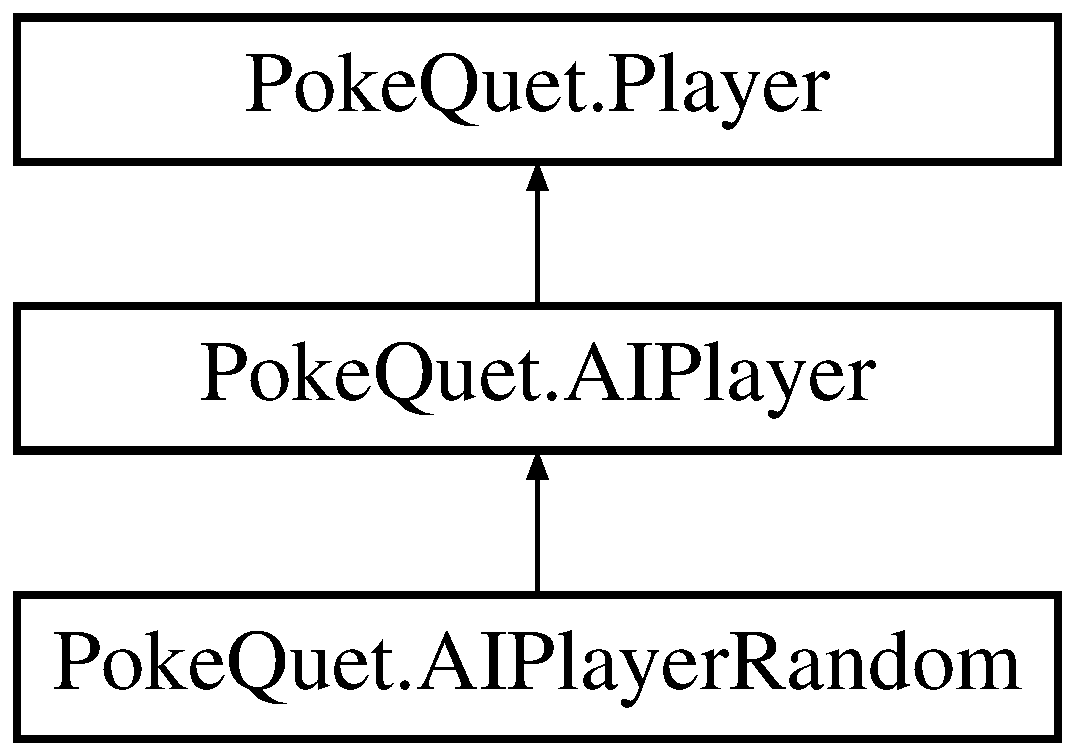
\includegraphics[height=3.000000cm]{class_poke_quet_1_1_a_i_player_random}
\end{center}
\end{figure}
\subsection*{Public Member Functions}
\begin{DoxyCompactItemize}
\item 
override \mbox{\hyperlink{namespace_poke_quet_aa425f1b8cf90847021fe1177d6a7199d}{Discipline}} \mbox{\hyperlink{class_poke_quet_1_1_a_i_player_random_a8723ee791e3ac1ea34033cd6ce49398f}{Make\+Turn}} (\mbox{\hyperlink{class_poke_quet_1_1_player}{Player}} opponent, \mbox{\hyperlink{class_poke_quet_1_1_deck}{Deck}} tie\+Cards)
\begin{DoxyCompactList}\small\item\em Die Methode zur Bestimmung des Zugs des Computerspielers \end{DoxyCompactList}\end{DoxyCompactItemize}
\subsection*{Additional Inherited Members}


\subsection{Detailed Description}
KI für leichten Computergegner, der völlig zufällige Disziplinen auswählt. 



\subsection{Member Function Documentation}
\mbox{\Hypertarget{class_poke_quet_1_1_a_i_player_random_a8723ee791e3ac1ea34033cd6ce49398f}\label{class_poke_quet_1_1_a_i_player_random_a8723ee791e3ac1ea34033cd6ce49398f}} 
\index{Poke\+Quet\+::\+A\+I\+Player\+Random@{Poke\+Quet\+::\+A\+I\+Player\+Random}!Make\+Turn@{Make\+Turn}}
\index{Make\+Turn@{Make\+Turn}!Poke\+Quet\+::\+A\+I\+Player\+Random@{Poke\+Quet\+::\+A\+I\+Player\+Random}}
\subsubsection{\texorpdfstring{Make\+Turn()}{MakeTurn()}}
{\footnotesize\ttfamily override \mbox{\hyperlink{namespace_poke_quet_aa425f1b8cf90847021fe1177d6a7199d}{Discipline}} Poke\+Quet.\+A\+I\+Player\+Random.\+Make\+Turn (\begin{DoxyParamCaption}\item[{\mbox{\hyperlink{class_poke_quet_1_1_player}{Player}}}]{opponent,  }\item[{\mbox{\hyperlink{class_poke_quet_1_1_deck}{Deck}}}]{tie\+Cards }\end{DoxyParamCaption})\hspace{0.3cm}{\ttfamily [inline]}, {\ttfamily [virtual]}}



Die Methode zur Bestimmung des Zugs des Computerspielers 


\begin{DoxyParams}{Parameters}
{\em opponent} & Der gegnerische Spieler\\
\hline
{\em tie\+Cards} & Der Stich-\/\+Stapel\\
\hline
\end{DoxyParams}
\begin{DoxyReturn}{Returns}
Die Disziplin die als Zug gewählt wird.
\end{DoxyReturn}


Implements \mbox{\hyperlink{class_poke_quet_1_1_a_i_player_ae2862ead657c524614793ea4d3ebf80b}{Poke\+Quet.\+A\+I\+Player}}.



The documentation for this class was generated from the following file\+:\begin{DoxyCompactItemize}
\item 
Player.\+cs\end{DoxyCompactItemize}

\hypertarget{class_poke_quet_1_1_a_i_player_simple}{}\section{Poke\+Quet.\+A\+I\+Player\+Simple Class Reference}
\label{class_poke_quet_1_1_a_i_player_simple}\index{Poke\+Quet.\+A\+I\+Player\+Simple@{Poke\+Quet.\+A\+I\+Player\+Simple}}


KI für schweren Computergegner, der logische Entscheidungen trifft und immer den höchsten Wert wählt, aber Type ignoriert.  


Inheritance diagram for Poke\+Quet.\+A\+I\+Player\+Simple\+:\begin{figure}[H]
\begin{center}
\leavevmode
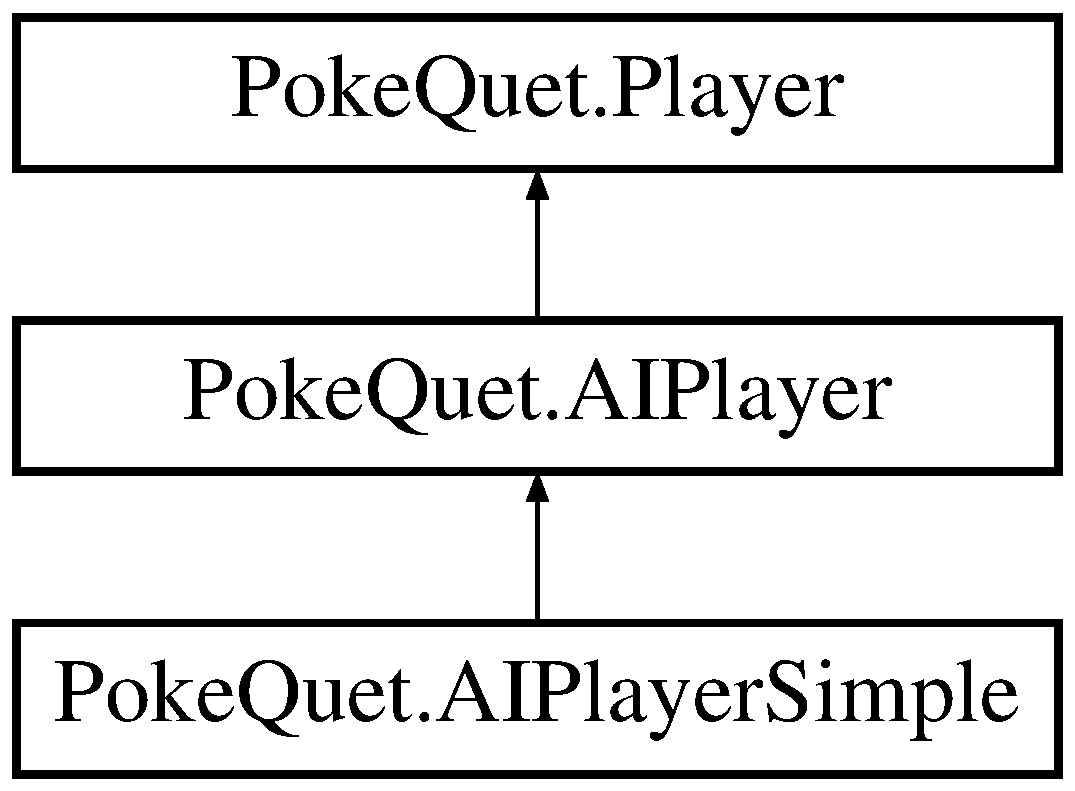
\includegraphics[height=3.000000cm]{class_poke_quet_1_1_a_i_player_simple}
\end{center}
\end{figure}
\subsection*{Public Member Functions}
\begin{DoxyCompactItemize}
\item 
override \mbox{\hyperlink{namespace_poke_quet_aa425f1b8cf90847021fe1177d6a7199d}{Discipline}} \mbox{\hyperlink{class_poke_quet_1_1_a_i_player_simple_a4c48360666f3fc8b7400cbfa2c7ea29e}{Make\+Turn}} (\mbox{\hyperlink{class_poke_quet_1_1_player}{Player}} opponent, \mbox{\hyperlink{class_poke_quet_1_1_deck}{Deck}} tie\+Cards)
\begin{DoxyCompactList}\small\item\em Die Methode zur Bestimmung des Zugs des Computerspielers \end{DoxyCompactList}\end{DoxyCompactItemize}
\subsection*{Additional Inherited Members}


\subsection{Detailed Description}
KI für schweren Computergegner, der logische Entscheidungen trifft und immer den höchsten Wert wählt, aber Type ignoriert. 



\subsection{Member Function Documentation}
\mbox{\Hypertarget{class_poke_quet_1_1_a_i_player_simple_a4c48360666f3fc8b7400cbfa2c7ea29e}\label{class_poke_quet_1_1_a_i_player_simple_a4c48360666f3fc8b7400cbfa2c7ea29e}} 
\index{Poke\+Quet\+::\+A\+I\+Player\+Simple@{Poke\+Quet\+::\+A\+I\+Player\+Simple}!Make\+Turn@{Make\+Turn}}
\index{Make\+Turn@{Make\+Turn}!Poke\+Quet\+::\+A\+I\+Player\+Simple@{Poke\+Quet\+::\+A\+I\+Player\+Simple}}
\subsubsection{\texorpdfstring{Make\+Turn()}{MakeTurn()}}
{\footnotesize\ttfamily override \mbox{\hyperlink{namespace_poke_quet_aa425f1b8cf90847021fe1177d6a7199d}{Discipline}} Poke\+Quet.\+A\+I\+Player\+Simple.\+Make\+Turn (\begin{DoxyParamCaption}\item[{\mbox{\hyperlink{class_poke_quet_1_1_player}{Player}}}]{opponent,  }\item[{\mbox{\hyperlink{class_poke_quet_1_1_deck}{Deck}}}]{tie\+Cards }\end{DoxyParamCaption})\hspace{0.3cm}{\ttfamily [inline]}, {\ttfamily [virtual]}}



Die Methode zur Bestimmung des Zugs des Computerspielers 


\begin{DoxyParams}{Parameters}
{\em opponent} & Der gegnerische Spieler\\
\hline
{\em tie\+Cards} & Der Stich-\/\+Stapel\\
\hline
\end{DoxyParams}
\begin{DoxyReturn}{Returns}
Die Disziplin die als Zug gewählt wird.
\end{DoxyReturn}


Implements \mbox{\hyperlink{class_poke_quet_1_1_a_i_player_ae2862ead657c524614793ea4d3ebf80b}{Poke\+Quet.\+A\+I\+Player}}.



The documentation for this class was generated from the following file\+:\begin{DoxyCompactItemize}
\item 
Player.\+cs\end{DoxyCompactItemize}

\hypertarget{class_poke_quet_1_1_card}{}\section{Poke\+Quet.\+Card Class Reference}
\label{class_poke_quet_1_1_card}\index{Poke\+Quet.\+Card@{Poke\+Quet.\+Card}}


Klasse die eine Karte darstellt und durch Modelbinding via J\+S\+O\+N.\+N\+ET zusammengebaut wird.  


\subsection*{Public Attributes}
\begin{DoxyCompactItemize}
\item 
\mbox{\Hypertarget{class_poke_quet_1_1_card_a07bbff6c7bf7c020375b5f227c7ec9d8}\label{class_poke_quet_1_1_card_a07bbff6c7bf7c020375b5f227c7ec9d8}} 
string {\bfseries name}
\item 
\mbox{\Hypertarget{class_poke_quet_1_1_card_a5486c0c3f0a4450716fa1bf092f1793a}\label{class_poke_quet_1_1_card_a5486c0c3f0a4450716fa1bf092f1793a}} 
int {\bfseries hp}
\end{DoxyCompactItemize}


\subsection{Detailed Description}
Klasse die eine Karte darstellt und durch Modelbinding via J\+S\+O\+N.\+N\+ET zusammengebaut wird. 



The documentation for this class was generated from the following file\+:\begin{DoxyCompactItemize}
\item 
Card.\+cs\end{DoxyCompactItemize}

\hypertarget{class_poke_quet_1_1_deck}{}\section{Poke\+Quet.\+Deck Class Reference}
\label{class_poke_quet_1_1_deck}\index{Poke\+Quet.\+Deck@{Poke\+Quet.\+Deck}}


Klasse die ein Kartendeck darstellt und keine  


Inheritance diagram for Poke\+Quet.\+Deck\+:\begin{figure}[H]
\begin{center}
\leavevmode
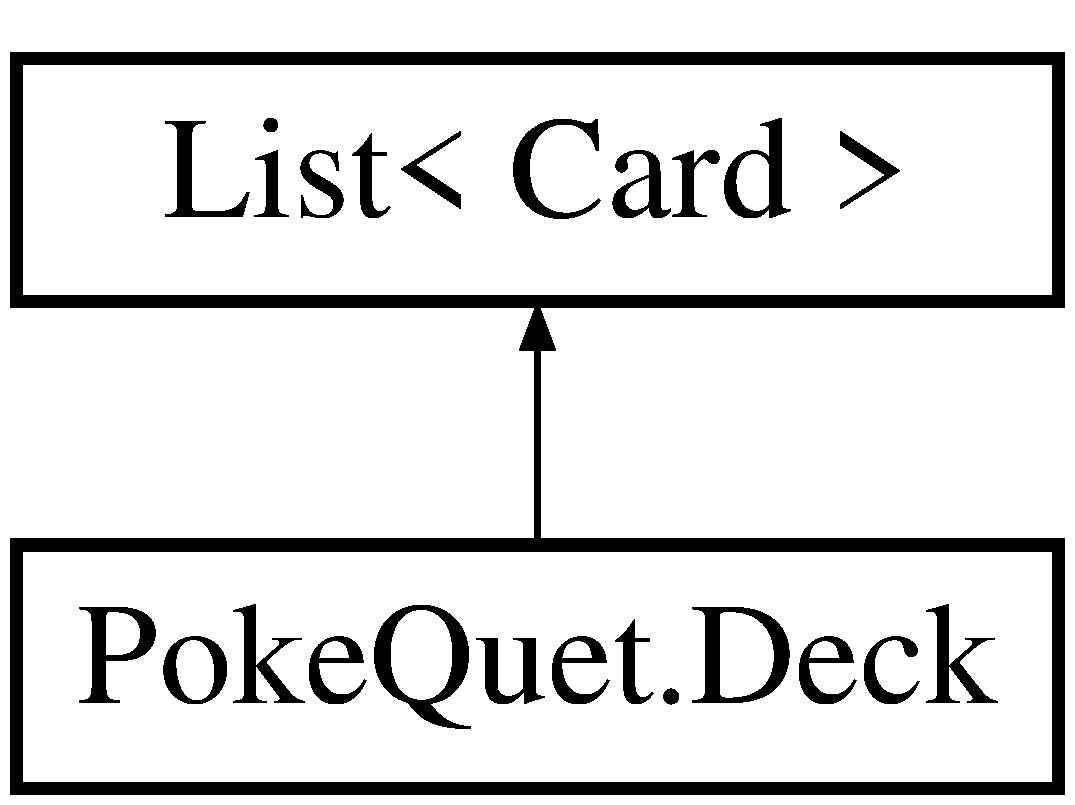
\includegraphics[height=2.000000cm]{class_poke_quet_1_1_deck}
\end{center}
\end{figure}
\subsection*{Public Member Functions}
\begin{DoxyCompactItemize}
\item 
\mbox{\hyperlink{class_poke_quet_1_1_card}{Card}} \mbox{\hyperlink{class_poke_quet_1_1_deck_a54d648dd64cb769d6817cc4bcf0e9af2}{Get\+Current\+Card}} ()
\begin{DoxyCompactList}\small\item\em Gibt die aktuelle(vorderste) Karte des Decks zurück. Im wesentlichen nur eine Wrapperfunktion, die dazu da ist Listenoperationen durch Analogien aus dem echten Leben verständlicher zu machen. \end{DoxyCompactList}\item 
void \mbox{\hyperlink{class_poke_quet_1_1_deck_a48673ad29ddff99adc0d494192d5f47c}{Put\+Cards\+At\+Back}} (I\+Enumerable$<$ \mbox{\hyperlink{class_poke_quet_1_1_card}{Card}} $>$ cards)
\begin{DoxyCompactList}\small\item\em Packt eine Menge an Karten hinten auf das \mbox{\hyperlink{class_poke_quet_1_1_deck}{Deck}}. Im wesentlichen nur eine Wrapperfunktion, die dazu da ist Listenoperationen durch Analogien aus dem echten Leben verständlicher zu machen. \end{DoxyCompactList}\item 
void \mbox{\hyperlink{class_poke_quet_1_1_deck_ae72396d102166a59850288ccb5be7fd1}{Put\+Cards\+At\+Back}} (params \mbox{\hyperlink{class_poke_quet_1_1_card}{Card}}\mbox{[}$\,$\mbox{]} cards)
\begin{DoxyCompactList}\small\item\em Packt eine Menge an Karten hinten auf das \mbox{\hyperlink{class_poke_quet_1_1_deck}{Deck}}. Implementiert um params-\/\+Aufrufe zu ermöglichen. Im wesentlichen nur eine Wrapperfunktion, die dazu da ist Listenoperationen durch Analogien aus dem echten Leben verständlicher zu machen. \end{DoxyCompactList}\end{DoxyCompactItemize}
\subsection*{Static Public Member Functions}
\begin{DoxyCompactItemize}
\item 
static void \mbox{\hyperlink{class_poke_quet_1_1_deck_a12d9b5d3adc4c8c129f04ad024000a0c}{Fill\+Decks\+From\+Card\+Pool}} (\mbox{\hyperlink{class_poke_quet_1_1_card}{Card}}\mbox{[}$\,$\mbox{]} pool, \mbox{\hyperlink{class_poke_quet_1_1_deck}{Deck}} deck1, \mbox{\hyperlink{class_poke_quet_1_1_deck}{Deck}} deck2, int deck\+Size)
\begin{DoxyCompactList}\small\item\em Packt eine Menge an Karten hinten auf das \mbox{\hyperlink{class_poke_quet_1_1_deck}{Deck}}. Implementiert um params-\/\+Aufrufe zu ermöglichen. Im wesentlichen nur eine Wrapperfunktion, die dazu da ist Listenoperationen durch Analogien aus dem echten Leben verständlicher zu machen. \end{DoxyCompactList}\end{DoxyCompactItemize}
\subsection*{Static Public Attributes}
\begin{DoxyCompactItemize}
\item 
\mbox{\Hypertarget{class_poke_quet_1_1_deck_a3a9710bea0016f80f89e0160717b457f}\label{class_poke_quet_1_1_deck_a3a9710bea0016f80f89e0160717b457f}} 
static readonly Random {\bfseries R\+NG} = new Random()
\end{DoxyCompactItemize}


\subsection{Detailed Description}
Klasse die ein Kartendeck darstellt und keine 



\subsection{Member Function Documentation}
\mbox{\Hypertarget{class_poke_quet_1_1_deck_a12d9b5d3adc4c8c129f04ad024000a0c}\label{class_poke_quet_1_1_deck_a12d9b5d3adc4c8c129f04ad024000a0c}} 
\index{Poke\+Quet\+::\+Deck@{Poke\+Quet\+::\+Deck}!Fill\+Decks\+From\+Card\+Pool@{Fill\+Decks\+From\+Card\+Pool}}
\index{Fill\+Decks\+From\+Card\+Pool@{Fill\+Decks\+From\+Card\+Pool}!Poke\+Quet\+::\+Deck@{Poke\+Quet\+::\+Deck}}
\subsubsection{\texorpdfstring{Fill\+Decks\+From\+Card\+Pool()}{FillDecksFromCardPool()}}
{\footnotesize\ttfamily static void Poke\+Quet.\+Deck.\+Fill\+Decks\+From\+Card\+Pool (\begin{DoxyParamCaption}\item[{\mbox{\hyperlink{class_poke_quet_1_1_card}{Card}} \mbox{[}$\,$\mbox{]}}]{pool,  }\item[{\mbox{\hyperlink{class_poke_quet_1_1_deck}{Deck}}}]{deck1,  }\item[{\mbox{\hyperlink{class_poke_quet_1_1_deck}{Deck}}}]{deck2,  }\item[{int}]{deck\+Size }\end{DoxyParamCaption})\hspace{0.3cm}{\ttfamily [inline]}, {\ttfamily [static]}}



Packt eine Menge an Karten hinten auf das \mbox{\hyperlink{class_poke_quet_1_1_deck}{Deck}}. Implementiert um params-\/\+Aufrufe zu ermöglichen. Im wesentlichen nur eine Wrapperfunktion, die dazu da ist Listenoperationen durch Analogien aus dem echten Leben verständlicher zu machen. 

\begin{DoxyReturn}{Returns}
Die aktuelle Karte des Decks
\end{DoxyReturn}


Code von Tim und André\mbox{\Hypertarget{class_poke_quet_1_1_deck_a54d648dd64cb769d6817cc4bcf0e9af2}\label{class_poke_quet_1_1_deck_a54d648dd64cb769d6817cc4bcf0e9af2}} 
\index{Poke\+Quet\+::\+Deck@{Poke\+Quet\+::\+Deck}!Get\+Current\+Card@{Get\+Current\+Card}}
\index{Get\+Current\+Card@{Get\+Current\+Card}!Poke\+Quet\+::\+Deck@{Poke\+Quet\+::\+Deck}}
\subsubsection{\texorpdfstring{Get\+Current\+Card()}{GetCurrentCard()}}
{\footnotesize\ttfamily \mbox{\hyperlink{class_poke_quet_1_1_card}{Card}} Poke\+Quet.\+Deck.\+Get\+Current\+Card (\begin{DoxyParamCaption}{ }\end{DoxyParamCaption})\hspace{0.3cm}{\ttfamily [inline]}}



Gibt die aktuelle(vorderste) Karte des Decks zurück. Im wesentlichen nur eine Wrapperfunktion, die dazu da ist Listenoperationen durch Analogien aus dem echten Leben verständlicher zu machen. 

\begin{DoxyReturn}{Returns}
Die aktuelle Karte des Decks
\end{DoxyReturn}


Code ausschließlich von André\mbox{\Hypertarget{class_poke_quet_1_1_deck_a48673ad29ddff99adc0d494192d5f47c}\label{class_poke_quet_1_1_deck_a48673ad29ddff99adc0d494192d5f47c}} 
\index{Poke\+Quet\+::\+Deck@{Poke\+Quet\+::\+Deck}!Put\+Cards\+At\+Back@{Put\+Cards\+At\+Back}}
\index{Put\+Cards\+At\+Back@{Put\+Cards\+At\+Back}!Poke\+Quet\+::\+Deck@{Poke\+Quet\+::\+Deck}}
\subsubsection{\texorpdfstring{Put\+Cards\+At\+Back()}{PutCardsAtBack()}\hspace{0.1cm}{\footnotesize\ttfamily [1/2]}}
{\footnotesize\ttfamily void Poke\+Quet.\+Deck.\+Put\+Cards\+At\+Back (\begin{DoxyParamCaption}\item[{I\+Enumerable$<$ \mbox{\hyperlink{class_poke_quet_1_1_card}{Card}} $>$}]{cards }\end{DoxyParamCaption})\hspace{0.3cm}{\ttfamily [inline]}}



Packt eine Menge an Karten hinten auf das \mbox{\hyperlink{class_poke_quet_1_1_deck}{Deck}}. Im wesentlichen nur eine Wrapperfunktion, die dazu da ist Listenoperationen durch Analogien aus dem echten Leben verständlicher zu machen. 

\begin{DoxyReturn}{Returns}
Die aktuelle Karte des Decks
\end{DoxyReturn}


Code ausschließlich von André\mbox{\Hypertarget{class_poke_quet_1_1_deck_ae72396d102166a59850288ccb5be7fd1}\label{class_poke_quet_1_1_deck_ae72396d102166a59850288ccb5be7fd1}} 
\index{Poke\+Quet\+::\+Deck@{Poke\+Quet\+::\+Deck}!Put\+Cards\+At\+Back@{Put\+Cards\+At\+Back}}
\index{Put\+Cards\+At\+Back@{Put\+Cards\+At\+Back}!Poke\+Quet\+::\+Deck@{Poke\+Quet\+::\+Deck}}
\subsubsection{\texorpdfstring{Put\+Cards\+At\+Back()}{PutCardsAtBack()}\hspace{0.1cm}{\footnotesize\ttfamily [2/2]}}
{\footnotesize\ttfamily void Poke\+Quet.\+Deck.\+Put\+Cards\+At\+Back (\begin{DoxyParamCaption}\item[{params \mbox{\hyperlink{class_poke_quet_1_1_card}{Card}} \mbox{[}$\,$\mbox{]}}]{cards }\end{DoxyParamCaption})\hspace{0.3cm}{\ttfamily [inline]}}



Packt eine Menge an Karten hinten auf das \mbox{\hyperlink{class_poke_quet_1_1_deck}{Deck}}. Implementiert um params-\/\+Aufrufe zu ermöglichen. Im wesentlichen nur eine Wrapperfunktion, die dazu da ist Listenoperationen durch Analogien aus dem echten Leben verständlicher zu machen. 

\begin{DoxyReturn}{Returns}
Die aktuelle Karte des Decks
\end{DoxyReturn}


Code ausschließlich von André

The documentation for this class was generated from the following file\+:\begin{DoxyCompactItemize}
\item 
Card.\+cs\end{DoxyCompactItemize}

\hypertarget{class_poke_quet_1_1_game_over_dialog}{}\section{Poke\+Quet.\+Game\+Over\+Dialog Class Reference}
\label{class_poke_quet_1_1_game_over_dialog}\index{Poke\+Quet.\+Game\+Over\+Dialog@{Poke\+Quet.\+Game\+Over\+Dialog}}


Fenster das nach Ende des Spiels erscheint und den Sieger bzw. Unentschieden anzeigt und die Option für Neustart oder Ende des aktuellen Spiels gibt  


Inheritance diagram for Poke\+Quet.\+Game\+Over\+Dialog\+:\begin{figure}[H]
\begin{center}
\leavevmode
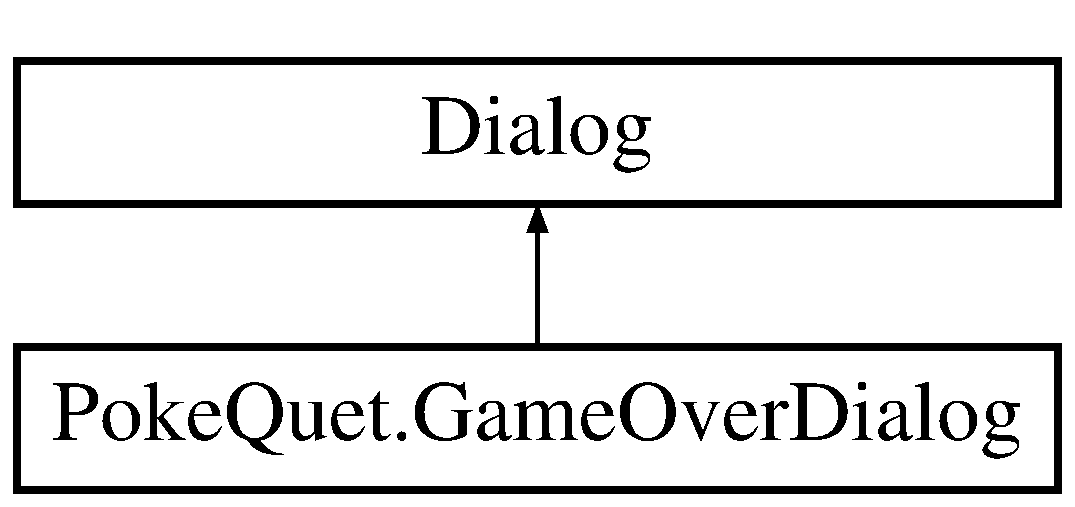
\includegraphics[height=2.000000cm]{class_poke_quet_1_1_game_over_dialog}
\end{center}
\end{figure}
\subsection*{Public Member Functions}
\begin{DoxyCompactItemize}
\item 
\mbox{\hyperlink{class_poke_quet_1_1_game_over_dialog_a8c93fc8093ac6012aa11d16bac7be605}{Game\+Over\+Dialog}} (\mbox{\hyperlink{class_main_window}{Main\+Window}} window, \mbox{\hyperlink{class_poke_quet_1_1_player}{Player}} winning\+Player, int player\+Num)
\begin{DoxyCompactList}\small\item\em Konstukter des Gameover-\/\+Dialogs welcher den Sieger bzw. Unentschieden anzeigt und die Option für Neustart oder Ende des aktuellen Spiels gibt \end{DoxyCompactList}\end{DoxyCompactItemize}
\subsection*{Public Attributes}
\begin{DoxyCompactItemize}
\item 
\mbox{\Hypertarget{class_poke_quet_1_1_game_over_dialog_a3da51964f7f1a7de547eae90f781429b}\label{class_poke_quet_1_1_game_over_dialog_a3da51964f7f1a7de547eae90f781429b}} 
const string {\bfseries P\+L\+A\+Y\+E\+R\+\_\+\+W\+ON} = \char`\"{}\{0\}(P\{1\}) W\+O\+N!\char`\"{}
\item 
\mbox{\Hypertarget{class_poke_quet_1_1_game_over_dialog_aa4ac065867974d1cabdf0b0fd8137a0a}\label{class_poke_quet_1_1_game_over_dialog_aa4ac065867974d1cabdf0b0fd8137a0a}} 
const string {\bfseries D\+R\+AW} = \char`\"{}D\+R\+A\+W!\char`\"{}
\end{DoxyCompactItemize}
\subsection*{Protected Member Functions}
\begin{DoxyCompactItemize}
\item 
void \mbox{\hyperlink{class_poke_quet_1_1_game_over_dialog_aa12eeeb856f3efec7e3bfff392a59af5}{Restart\+Clicked}} (object sender, Event\+Args e)
\begin{DoxyCompactList}\small\item\em Wenn Restart-\/\+Knopf gedrückt wird\+: Startet das Spiel neu und schließt den Dialog \end{DoxyCompactList}\item 
void \mbox{\hyperlink{class_poke_quet_1_1_game_over_dialog_a1f55fe2f8582123f180ceee6d4ea9150}{Quit\+Clicked}} (object sender, Event\+Args e)
\begin{DoxyCompactList}\small\item\em Wenn \char`\"{}\+Quit Game\char`\"{}-\/\+Knopf gedrückt wird\+: Schließt Fenster und beendet das Programm komplett \end{DoxyCompactList}\item 
void \mbox{\hyperlink{class_poke_quet_1_1_game_over_dialog_a17735956b84e755b1412e6a10ac92ed0}{On\+Button\+Main\+Menu\+Clicked}} (object sender, Event\+Args e)
\begin{DoxyCompactList}\small\item\em Wenn \char`\"{}\+Quit Game\char`\"{}-\/\+Knopf gedrückt wird\+: Schließt das Spiel Fenster und den Dialog, Das Hauptmenü bleibt offen \end{DoxyCompactList}\end{DoxyCompactItemize}


\subsection{Detailed Description}
Fenster das nach Ende des Spiels erscheint und den Sieger bzw. Unentschieden anzeigt und die Option für Neustart oder Ende des aktuellen Spiels gibt 



\subsection{Constructor \& Destructor Documentation}
\mbox{\Hypertarget{class_poke_quet_1_1_game_over_dialog_a8c93fc8093ac6012aa11d16bac7be605}\label{class_poke_quet_1_1_game_over_dialog_a8c93fc8093ac6012aa11d16bac7be605}} 
\index{Poke\+Quet\+::\+Game\+Over\+Dialog@{Poke\+Quet\+::\+Game\+Over\+Dialog}!Game\+Over\+Dialog@{Game\+Over\+Dialog}}
\index{Game\+Over\+Dialog@{Game\+Over\+Dialog}!Poke\+Quet\+::\+Game\+Over\+Dialog@{Poke\+Quet\+::\+Game\+Over\+Dialog}}
\subsubsection{\texorpdfstring{Game\+Over\+Dialog()}{GameOverDialog()}}
{\footnotesize\ttfamily Poke\+Quet.\+Game\+Over\+Dialog.\+Game\+Over\+Dialog (\begin{DoxyParamCaption}\item[{\mbox{\hyperlink{class_main_window}{Main\+Window}}}]{window,  }\item[{\mbox{\hyperlink{class_poke_quet_1_1_player}{Player}}}]{winning\+Player,  }\item[{int}]{player\+Num }\end{DoxyParamCaption})\hspace{0.3cm}{\ttfamily [inline]}}



Konstukter des Gameover-\/\+Dialogs welcher den Sieger bzw. Unentschieden anzeigt und die Option für Neustart oder Ende des aktuellen Spiels gibt 


\begin{DoxyParams}{Parameters}
{\em window} & Das Hauptspielfenster(benötigt für Neustart/\+Beendigung)\\
\hline
{\em winning\+Player} & Der Sieger des Spiels oder null falls Unentschieden\\
\hline
{\em player\+Num} & Die Zahl des Spielers der gewonnen hat(1 oder 2)\\
\hline
\end{DoxyParams}


Code von Tim und André

\subsection{Member Function Documentation}
\mbox{\Hypertarget{class_poke_quet_1_1_game_over_dialog_a17735956b84e755b1412e6a10ac92ed0}\label{class_poke_quet_1_1_game_over_dialog_a17735956b84e755b1412e6a10ac92ed0}} 
\index{Poke\+Quet\+::\+Game\+Over\+Dialog@{Poke\+Quet\+::\+Game\+Over\+Dialog}!On\+Button\+Main\+Menu\+Clicked@{On\+Button\+Main\+Menu\+Clicked}}
\index{On\+Button\+Main\+Menu\+Clicked@{On\+Button\+Main\+Menu\+Clicked}!Poke\+Quet\+::\+Game\+Over\+Dialog@{Poke\+Quet\+::\+Game\+Over\+Dialog}}
\subsubsection{\texorpdfstring{On\+Button\+Main\+Menu\+Clicked()}{OnButtonMainMenuClicked()}}
{\footnotesize\ttfamily void Poke\+Quet.\+Game\+Over\+Dialog.\+On\+Button\+Main\+Menu\+Clicked (\begin{DoxyParamCaption}\item[{object}]{sender,  }\item[{Event\+Args}]{e }\end{DoxyParamCaption})\hspace{0.3cm}{\ttfamily [inline]}, {\ttfamily [protected]}}



Wenn \char`\"{}\+Quit Game\char`\"{}-\/\+Knopf gedrückt wird\+: Schließt das Spiel Fenster und den Dialog, Das Hauptmenü bleibt offen 

Code ausschließlich von Tim\mbox{\Hypertarget{class_poke_quet_1_1_game_over_dialog_a1f55fe2f8582123f180ceee6d4ea9150}\label{class_poke_quet_1_1_game_over_dialog_a1f55fe2f8582123f180ceee6d4ea9150}} 
\index{Poke\+Quet\+::\+Game\+Over\+Dialog@{Poke\+Quet\+::\+Game\+Over\+Dialog}!Quit\+Clicked@{Quit\+Clicked}}
\index{Quit\+Clicked@{Quit\+Clicked}!Poke\+Quet\+::\+Game\+Over\+Dialog@{Poke\+Quet\+::\+Game\+Over\+Dialog}}
\subsubsection{\texorpdfstring{Quit\+Clicked()}{QuitClicked()}}
{\footnotesize\ttfamily void Poke\+Quet.\+Game\+Over\+Dialog.\+Quit\+Clicked (\begin{DoxyParamCaption}\item[{object}]{sender,  }\item[{Event\+Args}]{e }\end{DoxyParamCaption})\hspace{0.3cm}{\ttfamily [inline]}, {\ttfamily [protected]}}



Wenn \char`\"{}\+Quit Game\char`\"{}-\/\+Knopf gedrückt wird\+: Schließt Fenster und beendet das Programm komplett 

Code ausschließlich von Tim\mbox{\Hypertarget{class_poke_quet_1_1_game_over_dialog_aa12eeeb856f3efec7e3bfff392a59af5}\label{class_poke_quet_1_1_game_over_dialog_aa12eeeb856f3efec7e3bfff392a59af5}} 
\index{Poke\+Quet\+::\+Game\+Over\+Dialog@{Poke\+Quet\+::\+Game\+Over\+Dialog}!Restart\+Clicked@{Restart\+Clicked}}
\index{Restart\+Clicked@{Restart\+Clicked}!Poke\+Quet\+::\+Game\+Over\+Dialog@{Poke\+Quet\+::\+Game\+Over\+Dialog}}
\subsubsection{\texorpdfstring{Restart\+Clicked()}{RestartClicked()}}
{\footnotesize\ttfamily void Poke\+Quet.\+Game\+Over\+Dialog.\+Restart\+Clicked (\begin{DoxyParamCaption}\item[{object}]{sender,  }\item[{Event\+Args}]{e }\end{DoxyParamCaption})\hspace{0.3cm}{\ttfamily [inline]}, {\ttfamily [protected]}}



Wenn Restart-\/\+Knopf gedrückt wird\+: Startet das Spiel neu und schließt den Dialog 

Code ausschließlich von André

The documentation for this class was generated from the following file\+:\begin{DoxyCompactItemize}
\item 
Game\+Over\+Dialog.\+cs\end{DoxyCompactItemize}

\hypertarget{class_poke_quet_1_1_main_class}{}\section{Poke\+Quet.\+Main\+Class Class Reference}
\label{class_poke_quet_1_1_main_class}\index{Poke\+Quet.\+Main\+Class@{Poke\+Quet.\+Main\+Class}}
\subsection*{Static Public Member Functions}
\begin{DoxyCompactItemize}
\item 
\mbox{\Hypertarget{class_poke_quet_1_1_main_class_a2ee62877a52aedfd454133e9676efccb}\label{class_poke_quet_1_1_main_class_a2ee62877a52aedfd454133e9676efccb}} 
static void {\bfseries Main} (string\mbox{[}$\,$\mbox{]} args)
\end{DoxyCompactItemize}


The documentation for this class was generated from the following file\+:\begin{DoxyCompactItemize}
\item 
Program.\+cs\end{DoxyCompactItemize}

\hypertarget{class_poke_quet_1_1_main_menu}{}\section{Poke\+Quet.\+Main\+Menu Class Reference}
\label{class_poke_quet_1_1_main_menu}\index{Poke\+Quet.\+Main\+Menu@{Poke\+Quet.\+Main\+Menu}}
Inheritance diagram for Poke\+Quet.\+Main\+Menu\+:\begin{figure}[H]
\begin{center}
\leavevmode
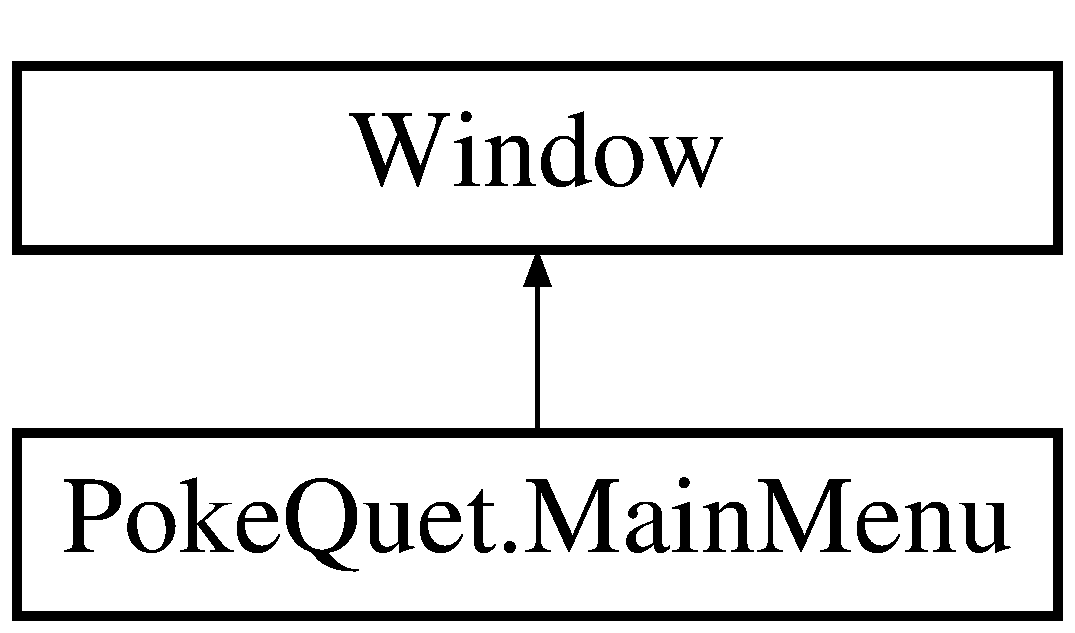
\includegraphics[height=2.000000cm]{class_poke_quet_1_1_main_menu}
\end{center}
\end{figure}
\subsection*{Protected Member Functions}
\begin{DoxyCompactItemize}
\item 
void \mbox{\hyperlink{class_poke_quet_1_1_main_menu_a66d3fc7a5c2b1b41fef3c3a1ee268c01}{Start\+Game\+Clicked}} (object sender, Event\+Args e)
\begin{DoxyCompactList}\small\item\em Wenn der \char`\"{}\+Start Game\char`\"{}-\/\+Knopf gedrückt wird eine neues Spiel mit den Einstellungen gestartet. \end{DoxyCompactList}\item 
void \mbox{\hyperlink{class_poke_quet_1_1_main_menu_a7838f72cbda854dda35ba2d309213646}{Quit\+Clicked}} (object sender, Event\+Args e)
\begin{DoxyCompactList}\small\item\em Wenn der \char`\"{}\+Quit\char`\"{}-\/\+Knopf gedrückt wird das komplette Programm geschlossen. \end{DoxyCompactList}\item 
\mbox{\Hypertarget{class_poke_quet_1_1_main_menu_ace589725732f2aeff8397f6a66741016}\label{class_poke_quet_1_1_main_menu_ace589725732f2aeff8397f6a66741016}} 
void {\bfseries On\+Delete\+Event} (object sender, Delete\+Event\+Args a)
\end{DoxyCompactItemize}


\subsection{Member Function Documentation}
\mbox{\Hypertarget{class_poke_quet_1_1_main_menu_a7838f72cbda854dda35ba2d309213646}\label{class_poke_quet_1_1_main_menu_a7838f72cbda854dda35ba2d309213646}} 
\index{Poke\+Quet\+::\+Main\+Menu@{Poke\+Quet\+::\+Main\+Menu}!Quit\+Clicked@{Quit\+Clicked}}
\index{Quit\+Clicked@{Quit\+Clicked}!Poke\+Quet\+::\+Main\+Menu@{Poke\+Quet\+::\+Main\+Menu}}
\subsubsection{\texorpdfstring{Quit\+Clicked()}{QuitClicked()}}
{\footnotesize\ttfamily void Poke\+Quet.\+Main\+Menu.\+Quit\+Clicked (\begin{DoxyParamCaption}\item[{object}]{sender,  }\item[{Event\+Args}]{e }\end{DoxyParamCaption})\hspace{0.3cm}{\ttfamily [inline]}, {\ttfamily [protected]}}



Wenn der \char`\"{}\+Quit\char`\"{}-\/\+Knopf gedrückt wird das komplette Programm geschlossen. 

\mbox{\Hypertarget{class_poke_quet_1_1_main_menu_a66d3fc7a5c2b1b41fef3c3a1ee268c01}\label{class_poke_quet_1_1_main_menu_a66d3fc7a5c2b1b41fef3c3a1ee268c01}} 
\index{Poke\+Quet\+::\+Main\+Menu@{Poke\+Quet\+::\+Main\+Menu}!Start\+Game\+Clicked@{Start\+Game\+Clicked}}
\index{Start\+Game\+Clicked@{Start\+Game\+Clicked}!Poke\+Quet\+::\+Main\+Menu@{Poke\+Quet\+::\+Main\+Menu}}
\subsubsection{\texorpdfstring{Start\+Game\+Clicked()}{StartGameClicked()}}
{\footnotesize\ttfamily void Poke\+Quet.\+Main\+Menu.\+Start\+Game\+Clicked (\begin{DoxyParamCaption}\item[{object}]{sender,  }\item[{Event\+Args}]{e }\end{DoxyParamCaption})\hspace{0.3cm}{\ttfamily [inline]}, {\ttfamily [protected]}}



Wenn der \char`\"{}\+Start Game\char`\"{}-\/\+Knopf gedrückt wird eine neues Spiel mit den Einstellungen gestartet. 



The documentation for this class was generated from the following file\+:\begin{DoxyCompactItemize}
\item 
Main\+Menu.\+cs\end{DoxyCompactItemize}

\hypertarget{class_main_window}{}\section{Main\+Window Class Reference}
\label{class_main_window}\index{Main\+Window@{Main\+Window}}


Das Hauptfenster (das Spiel)  


Inheritance diagram for Main\+Window\+:\begin{figure}[H]
\begin{center}
\leavevmode
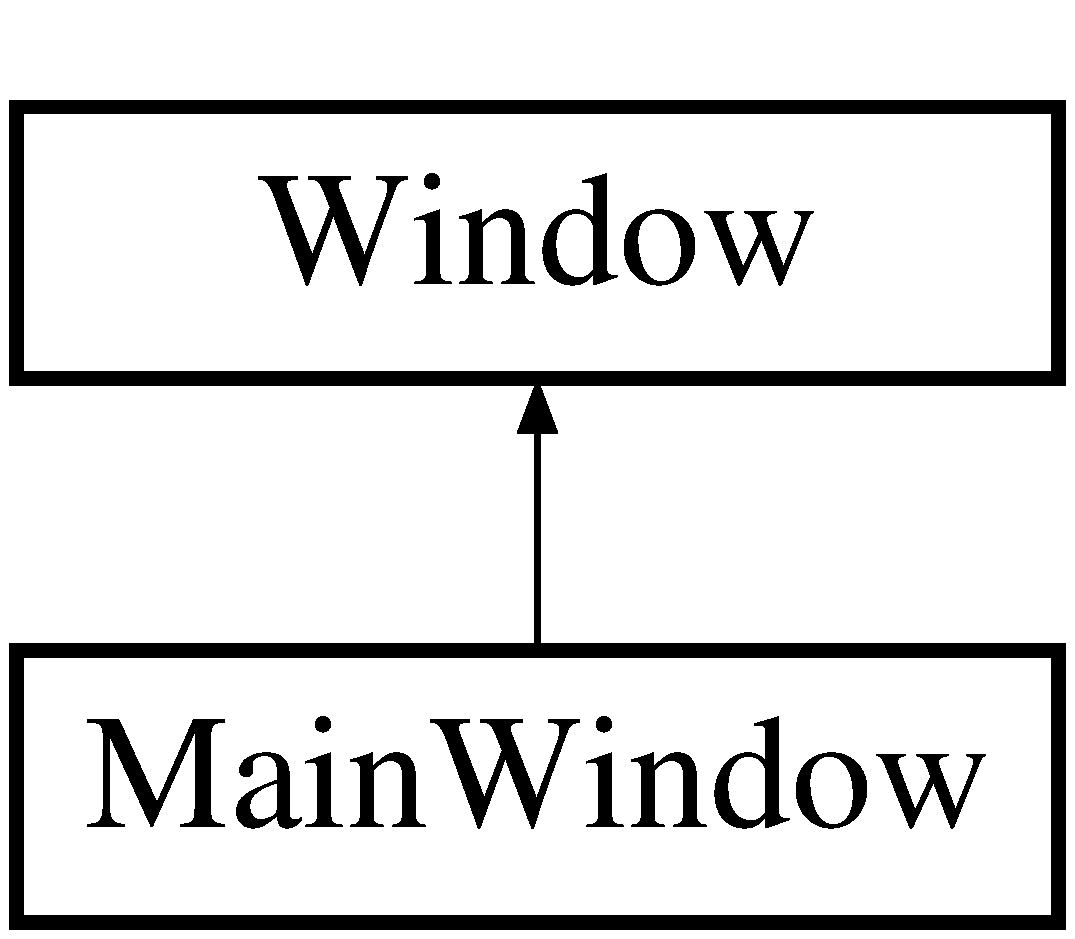
\includegraphics[height=2.000000cm]{class_main_window}
\end{center}
\end{figure}
\subsection*{Public Member Functions}
\begin{DoxyCompactItemize}
\item 
\mbox{\hyperlink{class_main_window_a159f4e738afbdf1dc79068aad1068725}{Main\+Window}} (string player\+Name, int ai\+Type, int starting\+Player, int deck\+Size)
\begin{DoxyCompactList}\small\item\em Konstruktor des Hauptfensters. Startet bereitet das Fenster vor und startet das Spiel. \end{DoxyCompactList}\item 
void \mbox{\hyperlink{class_main_window_afcb02d6059de11622938a544e3eda66a}{Init\+Game}} (string player\+Name, int ai\+Type)
\begin{DoxyCompactList}\small\item\em Initialisierung des Spiels\+: Laden der Karten, Erzeugung von Spielern auf Grundlage der gewählten KI, (Initialisierung der KI; obsolet) Erzeugung des Stich-\/\+Stapels Beginne Spiel \end{DoxyCompactList}\item 
void \mbox{\hyperlink{class_main_window_ad9f0cc9d0eafd2f12bbe701c1183450e}{Load\+Cards}} ()
\begin{DoxyCompactList}\small\item\em Lädt Karten aus der All\+Cards.\+json Datei und speicher sie in \mbox{\hyperlink{class_main_window_ae1c30b48118e2c8c6cd16171fab0cd31}{Card\+Pool}}. \end{DoxyCompactList}\item 
void \mbox{\hyperlink{class_main_window_a1eb0f2f5d231502046a64fef4a894a80}{Start\+Game}} ()
\begin{DoxyCompactList}\small\item\em Startet das Spiel\+: mischt und verteilt Decks, leert den Stich-\/\+Stapel, bestimmt den beginnenden Spieler, startet den ersten Zug \end{DoxyCompactList}\item 
void \mbox{\hyperlink{class_main_window_a66c105aa2c336bc2b05d9d574ab4eb74}{Next\+Turn}} ()
\begin{DoxyCompactList}\small\item\em Beginne einen neuen Zug\+: aktiviere Knöpfe falls Spieler 1 am Zug ist, mache C\+P\+U-\/\+Zug falls ein nicht-\/\+Spieler am Zug ist \end{DoxyCompactList}\item 
void \mbox{\hyperlink{class_main_window_ac527beb2a3d814c60578bd415c589dcf}{Display\+Cards}} ()
\begin{DoxyCompactList}\small\item\em Zeigt alle Informationen zur Karte von Spieler 1(die eigene) an; Leert die Informationen zur Karte von Spieler 2; Aktualisiert Kartenanzahlen für Decks; Stellt die normale Schriftfarbe der Disziplinen wieder her \end{DoxyCompactList}\item 
void \mbox{\hyperlink{class_main_window_ab0f20d9b5a33f6469d5b837799e534fc}{Choose\+Discipline}} (\mbox{\hyperlink{namespace_poke_quet_aa425f1b8cf90847021fe1177d6a7199d}{Discipline}} discipline)
\begin{DoxyCompactList}\small\item\em Wenn der Spieler eine Disziplin ausgewählt hat\+: Deaktiviere Disziplin-\/\+Knöpfe, Vergleiche Disziplin \end{DoxyCompactList}\item 
void \mbox{\hyperlink{class_main_window_a25b45e71a3e8fc76ab004cf4c9725c66}{Make\+C\+P\+U\+Move}} ()
\begin{DoxyCompactList}\small\item\em Mache den C\+P\+U-\/\+Zug (Spieler 2 macht seinen Zug) \end{DoxyCompactList}\item 
void \mbox{\hyperlink{class_main_window_a635fb220648803e533830c65bbe29fd8}{Show\+Opponent\+Card}} ()
\begin{DoxyCompactList}\small\item\em Aufdecken der aktuellen Karte und Werte von Spieler 2. Wird durch \mbox{\hyperlink{class_main_window_a4bbff733cfab680758c3fcc80a0de055}{Compare\+Discipline(\+Discipline)}} aufgerufen, nach Auswahl der Disziplin \end{DoxyCompactList}\item 
void \mbox{\hyperlink{class_main_window_aa29917f24b4b216e576a90b000db089d}{Show\+Turn\+Winner}} (\mbox{\hyperlink{namespace_poke_quet_aa425f1b8cf90847021fe1177d6a7199d}{Discipline}} discipline, \mbox{\hyperlink{class_poke_quet_1_1_player}{Player}} winning\+Player)
\begin{DoxyCompactList}\small\item\em Anzeige welcher Spieler die aktuelle Runde gewonnen hat\+: Färbt Kartenwerte der gewählten Disziplin ein, Zeigt Gewinner über \char`\"{}\+Next Card\char`\"{}-\/\+Knopf an \end{DoxyCompactList}\item 
void \mbox{\hyperlink{class_main_window_a4bbff733cfab680758c3fcc80a0de055}{Compare\+Discipline}} (\mbox{\hyperlink{namespace_poke_quet_aa425f1b8cf90847021fe1177d6a7199d}{Discipline}} discipline)
\begin{DoxyCompactList}\small\item\em Kampflogik\+: Vergleicht ausgewählte Disziplinen und entscheidet welcher Spieler die aktuelle Runde gewinnt oder ob es unentschieden endet. \end{DoxyCompactList}\item 
void \mbox{\hyperlink{class_main_window_a94a1278f08f427a805ea3fedf760e03c}{Round\+Decided}} (\mbox{\hyperlink{class_poke_quet_1_1_player}{Player}} winning\+Player, \mbox{\hyperlink{class_poke_quet_1_1_player}{Player}} losing\+Player, \mbox{\hyperlink{namespace_poke_quet_aa425f1b8cf90847021fe1177d6a7199d}{Discipline}} discipline)
\begin{DoxyCompactList}\small\item\em Nach dem die Runde entschieden wurde\+: Entfernt die beiden Karten der aktuellen Runde aus den Decks und fügt sie dem Deck des Gewinners hinzu, bzw. bei einem Unentschieden werden die Karten den \mbox{\hyperlink{class_main_window_a71f4eaa448a91297c8c54786e5c0516e}{Tie\+Cards}} hinzugefügt; Weise dem \mbox{\hyperlink{class_main_window_a4ce463cb4e7d116640b55416557ea741}{Active\+Player}} den Gewinner der aktuellen Runde zu (Der Gewinner ist als nächster am Zug.); Überprüfe ob das Spiel zuende ist durch einen Aufruf von \mbox{\hyperlink{class_main_window_a74ec52917be1fdf6a641639d5da39d53}{Check\+Winning\+State}} \end{DoxyCompactList}\item 
void \mbox{\hyperlink{class_main_window_a74ec52917be1fdf6a641639d5da39d53}{Check\+Winning\+State}} ()
\begin{DoxyCompactList}\small\item\em Überprüft anhand der verbleibenden Karten in den Decks, ob ein Spieler das Spiel gewonnen hat, oder ob das Spiel unentschieden endet. \end{DoxyCompactList}\end{DoxyCompactItemize}
\subsection*{Public Attributes}
\begin{DoxyCompactItemize}
\item 
\mbox{\Hypertarget{class_main_window_ae149b6fbe2080c77fe7bf34880fe4b15}\label{class_main_window_ae149b6fbe2080c77fe7bf34880fe4b15}} 
const string {\bfseries T\+U\+R\+N\+\_\+\+R\+E\+S\+U\+L\+T\+\_\+\+W\+I\+N\+N\+ER} = \char`\"{}\{0\} won the turn!\char`\"{}
\item 
\mbox{\Hypertarget{class_main_window_a678df4fce522ee399f2d91901da72004}\label{class_main_window_a678df4fce522ee399f2d91901da72004}} 
const string {\bfseries T\+U\+R\+N\+\_\+\+R\+E\+S\+U\+L\+T\+\_\+\+T\+IE} = \char`\"{}It\textquotesingle{}s a tie!\char`\"{}
\end{DoxyCompactItemize}
\subsection*{Static Public Attributes}
\begin{DoxyCompactItemize}
\item 
\mbox{\Hypertarget{class_main_window_a1ddfc1a8ba6354a1a9d29fa8ba942caa}\label{class_main_window_a1ddfc1a8ba6354a1a9d29fa8ba942caa}} 
static readonly Random {\bfseries R\+NG} = new Random()
\item 
\mbox{\Hypertarget{class_main_window_ad3cdf380f793df7d8df3632b8073093d}\label{class_main_window_ad3cdf380f793df7d8df3632b8073093d}} 
static readonly Gdk.\+Color {\bfseries R\+ED} = new Gdk.\+Color((byte)255, (byte)20, (byte)20)
\item 
\mbox{\Hypertarget{class_main_window_abf9286e51d9c9868c1d1c420383bc146}\label{class_main_window_abf9286e51d9c9868c1d1c420383bc146}} 
static readonly Gdk.\+Color {\bfseries G\+R\+E\+EN} = new Gdk.\+Color((byte)0, (byte)215, (byte)0)
\item 
\mbox{\Hypertarget{class_main_window_ac8dc783760d112de13cd19cffa89e51e}\label{class_main_window_ac8dc783760d112de13cd19cffa89e51e}} 
static readonly Gdk.\+Color {\bfseries G\+R\+EY} = new Gdk.\+Color((byte)0, (byte)0, (byte)0)
\item 
\mbox{\Hypertarget{class_main_window_af583645658035054e22a48ba2e29fa61}\label{class_main_window_af583645658035054e22a48ba2e29fa61}} 
static readonly Gdk.\+Color {\bfseries B\+L\+A\+CK} = new Gdk.\+Color((byte)0, (byte)0, (byte)0)
\end{DoxyCompactItemize}
\subsection*{Protected Member Functions}
\begin{DoxyCompactItemize}
\item 
void \mbox{\hyperlink{class_main_window_a148f7bce0a5842ae629b21de2516e585}{Next\+Card\+Clicked}} (object sender, Event\+Args e)
\begin{DoxyCompactList}\small\item\em Wenn der Spieler auf den \char`\"{}\+Next Card\char`\"{}-\/\+Knopf drückt\+: Beginne den nächsten Zug \end{DoxyCompactList}\item 
\mbox{\Hypertarget{class_main_window_ad015c2c419d25830d71dcaac0f97b199}\label{class_main_window_ad015c2c419d25830d71dcaac0f97b199}} 
void {\bfseries Type\+Discipline\+Selected} (object sender, Event\+Args e)
\item 
\mbox{\Hypertarget{class_main_window_a4adf98b53f1040dab240bcb004c88342}\label{class_main_window_a4adf98b53f1040dab240bcb004c88342}} 
void {\bfseries H\+P\+Discipline\+Selected} (object sender, Event\+Args e)
\item 
\mbox{\Hypertarget{class_main_window_a1d3d2bb960da9925ef3c85b3f5fbef42}\label{class_main_window_a1d3d2bb960da9925ef3c85b3f5fbef42}} 
void {\bfseries A\+T\+K\+Discipline\+Selected} (object sender, Event\+Args e)
\item 
\mbox{\Hypertarget{class_main_window_add34c6d17740a7e065c6d1bededaf145}\label{class_main_window_add34c6d17740a7e065c6d1bededaf145}} 
void {\bfseries D\+E\+F\+Discipline\+Selected} (object sender, Event\+Args e)
\item 
\mbox{\Hypertarget{class_main_window_af0fbe61daf0feaf38240ffca739f4a88}\label{class_main_window_af0fbe61daf0feaf38240ffca739f4a88}} 
void {\bfseries S\+P\+D\+Discipline\+Selected} (object sender, Event\+Args e)
\end{DoxyCompactItemize}
\subsection*{Properties}
\begin{DoxyCompactItemize}
\item 
\mbox{\hyperlink{class_poke_quet_1_1_card}{Card}} \mbox{[}$\,$\mbox{]} \mbox{\hyperlink{class_main_window_ae1c30b48118e2c8c6cd16171fab0cd31}{Card\+Pool}}\hspace{0.3cm}{\ttfamily  \mbox{[}get, set\mbox{]}}
\begin{DoxyCompactList}\small\item\em Array aller geladenen Karten \end{DoxyCompactList}\item 
\mbox{\hyperlink{class_poke_quet_1_1_player}{Player}} \mbox{\hyperlink{class_main_window_a4ce463cb4e7d116640b55416557ea741}{Active\+Player}}\hspace{0.3cm}{\ttfamily  \mbox{[}get, set\mbox{]}}
\begin{DoxyCompactList}\small\item\em Der aktive Spieler(= der Spieler der am Zug ist) \end{DoxyCompactList}\item 
\mbox{\Hypertarget{class_main_window_a49ed88cd1ccd49cb4489fd432ac6efa5}\label{class_main_window_a49ed88cd1ccd49cb4489fd432ac6efa5}} 
\mbox{\hyperlink{class_poke_quet_1_1_player}{Player}} {\bfseries Player1}\hspace{0.3cm}{\ttfamily  \mbox{[}get, set\mbox{]}}
\item 
\mbox{\Hypertarget{class_main_window_aed5200384ee8a791a584c07ae034b0d6}\label{class_main_window_aed5200384ee8a791a584c07ae034b0d6}} 
\mbox{\hyperlink{class_poke_quet_1_1_a_i_player}{A\+I\+Player}} {\bfseries Player2}\hspace{0.3cm}{\ttfamily  \mbox{[}get, set\mbox{]}}
\item 
\mbox{\hyperlink{class_poke_quet_1_1_deck}{Deck}} \mbox{\hyperlink{class_main_window_a71f4eaa448a91297c8c54786e5c0516e}{Tie\+Cards}}\hspace{0.3cm}{\ttfamily  \mbox{[}get, set\mbox{]}}
\begin{DoxyCompactList}\small\item\em Der Stich-\/\+Stapel \end{DoxyCompactList}\end{DoxyCompactItemize}


\subsection{Detailed Description}
Das Hauptfenster (das Spiel) 



\subsection{Constructor \& Destructor Documentation}
\mbox{\Hypertarget{class_main_window_a159f4e738afbdf1dc79068aad1068725}\label{class_main_window_a159f4e738afbdf1dc79068aad1068725}} 
\index{Main\+Window@{Main\+Window}!Main\+Window@{Main\+Window}}
\index{Main\+Window@{Main\+Window}!Main\+Window@{Main\+Window}}
\subsubsection{\texorpdfstring{Main\+Window()}{MainWindow()}}
{\footnotesize\ttfamily Main\+Window.\+Main\+Window (\begin{DoxyParamCaption}\item[{string}]{player\+Name,  }\item[{int}]{ai\+Type,  }\item[{int}]{starting\+Player,  }\item[{int}]{deck\+Size }\end{DoxyParamCaption})\hspace{0.3cm}{\ttfamily [inline]}}



Konstruktor des Hauptfensters. Startet bereitet das Fenster vor und startet das Spiel. 


\begin{DoxyParams}{Parameters}
{\em player\+Name} & Name für Spieler 1\\
\hline
{\em ai\+Type} & K\+I-\/\+Level\+: 1=Bug Catcher(\+Zufall), 2=Gym Leader(höchster Wert)\\
\hline
{\em starting\+Player} & Beginnender Spieler\+: 1$\vert$2\+: Spieler 1$\vert$2, 0\+: Zufall\\
\hline
{\em deck\+Size} & Anfängliche Deckgröße der Spieler\\
\hline
\end{DoxyParams}


\subsection{Member Function Documentation}
\mbox{\Hypertarget{class_main_window_a74ec52917be1fdf6a641639d5da39d53}\label{class_main_window_a74ec52917be1fdf6a641639d5da39d53}} 
\index{Main\+Window@{Main\+Window}!Check\+Winning\+State@{Check\+Winning\+State}}
\index{Check\+Winning\+State@{Check\+Winning\+State}!Main\+Window@{Main\+Window}}
\subsubsection{\texorpdfstring{Check\+Winning\+State()}{CheckWinningState()}}
{\footnotesize\ttfamily void Main\+Window.\+Check\+Winning\+State (\begin{DoxyParamCaption}{ }\end{DoxyParamCaption})\hspace{0.3cm}{\ttfamily [inline]}}



Überprüft anhand der verbleibenden Karten in den Decks, ob ein Spieler das Spiel gewonnen hat, oder ob das Spiel unentschieden endet. 

Code fast ausschließlich von Tim\mbox{\Hypertarget{class_main_window_ab0f20d9b5a33f6469d5b837799e534fc}\label{class_main_window_ab0f20d9b5a33f6469d5b837799e534fc}} 
\index{Main\+Window@{Main\+Window}!Choose\+Discipline@{Choose\+Discipline}}
\index{Choose\+Discipline@{Choose\+Discipline}!Main\+Window@{Main\+Window}}
\subsubsection{\texorpdfstring{Choose\+Discipline()}{ChooseDiscipline()}}
{\footnotesize\ttfamily void Main\+Window.\+Choose\+Discipline (\begin{DoxyParamCaption}\item[{\mbox{\hyperlink{namespace_poke_quet_aa425f1b8cf90847021fe1177d6a7199d}{Discipline}}}]{discipline }\end{DoxyParamCaption})\hspace{0.3cm}{\ttfamily [inline]}}



Wenn der Spieler eine Disziplin ausgewählt hat\+: Deaktiviere Disziplin-\/\+Knöpfe, Vergleiche Disziplin 


\begin{DoxyParams}{Parameters}
{\em discipline} & Die gewählte Disziplin\\
\hline
\end{DoxyParams}


Code ausschließlich von André\mbox{\Hypertarget{class_main_window_a4bbff733cfab680758c3fcc80a0de055}\label{class_main_window_a4bbff733cfab680758c3fcc80a0de055}} 
\index{Main\+Window@{Main\+Window}!Compare\+Discipline@{Compare\+Discipline}}
\index{Compare\+Discipline@{Compare\+Discipline}!Main\+Window@{Main\+Window}}
\subsubsection{\texorpdfstring{Compare\+Discipline()}{CompareDiscipline()}}
{\footnotesize\ttfamily void Main\+Window.\+Compare\+Discipline (\begin{DoxyParamCaption}\item[{\mbox{\hyperlink{namespace_poke_quet_aa425f1b8cf90847021fe1177d6a7199d}{Discipline}}}]{discipline }\end{DoxyParamCaption})\hspace{0.3cm}{\ttfamily [inline]}}



Kampflogik\+: Vergleicht ausgewählte Disziplinen und entscheidet welcher Spieler die aktuelle Runde gewinnt oder ob es unentschieden endet. 


\begin{DoxyParams}{Parameters}
{\em discipline} & \\
\hline
\end{DoxyParams}


Code fast ausschließlich von Tim\mbox{\Hypertarget{class_main_window_ac527beb2a3d814c60578bd415c589dcf}\label{class_main_window_ac527beb2a3d814c60578bd415c589dcf}} 
\index{Main\+Window@{Main\+Window}!Display\+Cards@{Display\+Cards}}
\index{Display\+Cards@{Display\+Cards}!Main\+Window@{Main\+Window}}
\subsubsection{\texorpdfstring{Display\+Cards()}{DisplayCards()}}
{\footnotesize\ttfamily void Main\+Window.\+Display\+Cards (\begin{DoxyParamCaption}{ }\end{DoxyParamCaption})\hspace{0.3cm}{\ttfamily [inline]}}



Zeigt alle Informationen zur Karte von Spieler 1(die eigene) an; Leert die Informationen zur Karte von Spieler 2; Aktualisiert Kartenanzahlen für Decks; Stellt die normale Schriftfarbe der Disziplinen wieder her 

Code ausschließlich von André\mbox{\Hypertarget{class_main_window_afcb02d6059de11622938a544e3eda66a}\label{class_main_window_afcb02d6059de11622938a544e3eda66a}} 
\index{Main\+Window@{Main\+Window}!Init\+Game@{Init\+Game}}
\index{Init\+Game@{Init\+Game}!Main\+Window@{Main\+Window}}
\subsubsection{\texorpdfstring{Init\+Game()}{InitGame()}}
{\footnotesize\ttfamily void Main\+Window.\+Init\+Game (\begin{DoxyParamCaption}\item[{string}]{player\+Name,  }\item[{int}]{ai\+Type }\end{DoxyParamCaption})\hspace{0.3cm}{\ttfamily [inline]}}



Initialisierung des Spiels\+: Laden der Karten, Erzeugung von Spielern auf Grundlage der gewählten KI, (Initialisierung der KI; obsolet) Erzeugung des Stich-\/\+Stapels Beginne Spiel 


\begin{DoxyParams}{Parameters}
{\em player\+Name} & Name für Spieler 1\\
\hline
{\em ai\+Type} & K\+I-\/\+Level\+: 1=Bug Catcher(\+Zufall), 2=Gym Leader(höchster Wert)\\
\hline
\end{DoxyParams}


Code ausschließlich von André\mbox{\Hypertarget{class_main_window_ad9f0cc9d0eafd2f12bbe701c1183450e}\label{class_main_window_ad9f0cc9d0eafd2f12bbe701c1183450e}} 
\index{Main\+Window@{Main\+Window}!Load\+Cards@{Load\+Cards}}
\index{Load\+Cards@{Load\+Cards}!Main\+Window@{Main\+Window}}
\subsubsection{\texorpdfstring{Load\+Cards()}{LoadCards()}}
{\footnotesize\ttfamily void Main\+Window.\+Load\+Cards (\begin{DoxyParamCaption}{ }\end{DoxyParamCaption})\hspace{0.3cm}{\ttfamily [inline]}}



Lädt Karten aus der All\+Cards.\+json Datei und speicher sie in \mbox{\hyperlink{class_main_window_ae1c30b48118e2c8c6cd16171fab0cd31}{Card\+Pool}}. 

Code von Tim mit Hilfe von André(Generic-\/\+Syntax) auf Grundlage eines Beispiels in der J\+S\+O\+N.\+N\+ET Dokumentaion\mbox{\Hypertarget{class_main_window_a25b45e71a3e8fc76ab004cf4c9725c66}\label{class_main_window_a25b45e71a3e8fc76ab004cf4c9725c66}} 
\index{Main\+Window@{Main\+Window}!Make\+C\+P\+U\+Move@{Make\+C\+P\+U\+Move}}
\index{Make\+C\+P\+U\+Move@{Make\+C\+P\+U\+Move}!Main\+Window@{Main\+Window}}
\subsubsection{\texorpdfstring{Make\+C\+P\+U\+Move()}{MakeCPUMove()}}
{\footnotesize\ttfamily void Main\+Window.\+Make\+C\+P\+U\+Move (\begin{DoxyParamCaption}{ }\end{DoxyParamCaption})\hspace{0.3cm}{\ttfamily [inline]}}



Mache den C\+P\+U-\/\+Zug (Spieler 2 macht seinen Zug) 

\mbox{\Hypertarget{class_main_window_a148f7bce0a5842ae629b21de2516e585}\label{class_main_window_a148f7bce0a5842ae629b21de2516e585}} 
\index{Main\+Window@{Main\+Window}!Next\+Card\+Clicked@{Next\+Card\+Clicked}}
\index{Next\+Card\+Clicked@{Next\+Card\+Clicked}!Main\+Window@{Main\+Window}}
\subsubsection{\texorpdfstring{Next\+Card\+Clicked()}{NextCardClicked()}}
{\footnotesize\ttfamily void Main\+Window.\+Next\+Card\+Clicked (\begin{DoxyParamCaption}\item[{object}]{sender,  }\item[{Event\+Args}]{e }\end{DoxyParamCaption})\hspace{0.3cm}{\ttfamily [protected]}}



Wenn der Spieler auf den \char`\"{}\+Next Card\char`\"{}-\/\+Knopf drückt\+: Beginne den nächsten Zug 

Code ausschließlich von André\mbox{\Hypertarget{class_main_window_a66c105aa2c336bc2b05d9d574ab4eb74}\label{class_main_window_a66c105aa2c336bc2b05d9d574ab4eb74}} 
\index{Main\+Window@{Main\+Window}!Next\+Turn@{Next\+Turn}}
\index{Next\+Turn@{Next\+Turn}!Main\+Window@{Main\+Window}}
\subsubsection{\texorpdfstring{Next\+Turn()}{NextTurn()}}
{\footnotesize\ttfamily void Main\+Window.\+Next\+Turn (\begin{DoxyParamCaption}{ }\end{DoxyParamCaption})\hspace{0.3cm}{\ttfamily [inline]}}



Beginne einen neuen Zug\+: aktiviere Knöpfe falls Spieler 1 am Zug ist, mache C\+P\+U-\/\+Zug falls ein nicht-\/\+Spieler am Zug ist 

Code ausschließlich von André\mbox{\Hypertarget{class_main_window_a94a1278f08f427a805ea3fedf760e03c}\label{class_main_window_a94a1278f08f427a805ea3fedf760e03c}} 
\index{Main\+Window@{Main\+Window}!Round\+Decided@{Round\+Decided}}
\index{Round\+Decided@{Round\+Decided}!Main\+Window@{Main\+Window}}
\subsubsection{\texorpdfstring{Round\+Decided()}{RoundDecided()}}
{\footnotesize\ttfamily void Main\+Window.\+Round\+Decided (\begin{DoxyParamCaption}\item[{\mbox{\hyperlink{class_poke_quet_1_1_player}{Player}}}]{winning\+Player,  }\item[{\mbox{\hyperlink{class_poke_quet_1_1_player}{Player}}}]{losing\+Player,  }\item[{\mbox{\hyperlink{namespace_poke_quet_aa425f1b8cf90847021fe1177d6a7199d}{Discipline}}}]{discipline }\end{DoxyParamCaption})\hspace{0.3cm}{\ttfamily [inline]}}



Nach dem die Runde entschieden wurde\+: Entfernt die beiden Karten der aktuellen Runde aus den Decks und fügt sie dem Deck des Gewinners hinzu, bzw. bei einem Unentschieden werden die Karten den \mbox{\hyperlink{class_main_window_a71f4eaa448a91297c8c54786e5c0516e}{Tie\+Cards}} hinzugefügt; Weise dem \mbox{\hyperlink{class_main_window_a4ce463cb4e7d116640b55416557ea741}{Active\+Player}} den Gewinner der aktuellen Runde zu (Der Gewinner ist als nächster am Zug.); Überprüfe ob das Spiel zuende ist durch einen Aufruf von \mbox{\hyperlink{class_main_window_a74ec52917be1fdf6a641639d5da39d53}{Check\+Winning\+State}} 


\begin{DoxyParams}{Parameters}
{\em winning\+Player} & Der gewinnende Spieler\\
\hline
{\em losing\+Player} & Der verlierende Spieler\\
\hline
{\em discipline} & Die gespielte Disiplin\\
\hline
\end{DoxyParams}


Code fast ausschließlich von Tim\mbox{\Hypertarget{class_main_window_a635fb220648803e533830c65bbe29fd8}\label{class_main_window_a635fb220648803e533830c65bbe29fd8}} 
\index{Main\+Window@{Main\+Window}!Show\+Opponent\+Card@{Show\+Opponent\+Card}}
\index{Show\+Opponent\+Card@{Show\+Opponent\+Card}!Main\+Window@{Main\+Window}}
\subsubsection{\texorpdfstring{Show\+Opponent\+Card()}{ShowOpponentCard()}}
{\footnotesize\ttfamily void Main\+Window.\+Show\+Opponent\+Card (\begin{DoxyParamCaption}{ }\end{DoxyParamCaption})\hspace{0.3cm}{\ttfamily [inline]}}



Aufdecken der aktuellen Karte und Werte von Spieler 2. Wird durch \mbox{\hyperlink{class_main_window_a4bbff733cfab680758c3fcc80a0de055}{Compare\+Discipline(\+Discipline)}} aufgerufen, nach Auswahl der Disziplin 

Code ausschließlich von André\mbox{\Hypertarget{class_main_window_aa29917f24b4b216e576a90b000db089d}\label{class_main_window_aa29917f24b4b216e576a90b000db089d}} 
\index{Main\+Window@{Main\+Window}!Show\+Turn\+Winner@{Show\+Turn\+Winner}}
\index{Show\+Turn\+Winner@{Show\+Turn\+Winner}!Main\+Window@{Main\+Window}}
\subsubsection{\texorpdfstring{Show\+Turn\+Winner()}{ShowTurnWinner()}}
{\footnotesize\ttfamily void Main\+Window.\+Show\+Turn\+Winner (\begin{DoxyParamCaption}\item[{\mbox{\hyperlink{namespace_poke_quet_aa425f1b8cf90847021fe1177d6a7199d}{Discipline}}}]{discipline,  }\item[{\mbox{\hyperlink{class_poke_quet_1_1_player}{Player}}}]{winning\+Player }\end{DoxyParamCaption})\hspace{0.3cm}{\ttfamily [inline]}}



Anzeige welcher Spieler die aktuelle Runde gewonnen hat\+: Färbt Kartenwerte der gewählten Disziplin ein, Zeigt Gewinner über \char`\"{}\+Next Card\char`\"{}-\/\+Knopf an 


\begin{DoxyParams}{Parameters}
{\em discipline} & Die gewählte Disziplin zum Einfärben\\
\hline
{\em winning\+Player} & Der Spieler, der gewonnen hat oder null bei Unentschieden\\
\hline
\end{DoxyParams}


Code ausschließlich von André\mbox{\Hypertarget{class_main_window_a1eb0f2f5d231502046a64fef4a894a80}\label{class_main_window_a1eb0f2f5d231502046a64fef4a894a80}} 
\index{Main\+Window@{Main\+Window}!Start\+Game@{Start\+Game}}
\index{Start\+Game@{Start\+Game}!Main\+Window@{Main\+Window}}
\subsubsection{\texorpdfstring{Start\+Game()}{StartGame()}}
{\footnotesize\ttfamily void Main\+Window.\+Start\+Game (\begin{DoxyParamCaption}{ }\end{DoxyParamCaption})\hspace{0.3cm}{\ttfamily [inline]}}



Startet das Spiel\+: mischt und verteilt Decks, leert den Stich-\/\+Stapel, bestimmt den beginnenden Spieler, startet den ersten Zug 

Code fast ausschließlich von André

\subsection{Property Documentation}
\mbox{\Hypertarget{class_main_window_a4ce463cb4e7d116640b55416557ea741}\label{class_main_window_a4ce463cb4e7d116640b55416557ea741}} 
\index{Main\+Window@{Main\+Window}!Active\+Player@{Active\+Player}}
\index{Active\+Player@{Active\+Player}!Main\+Window@{Main\+Window}}
\subsubsection{\texorpdfstring{Active\+Player}{ActivePlayer}}
{\footnotesize\ttfamily \mbox{\hyperlink{class_poke_quet_1_1_player}{Player}} Main\+Window.\+Active\+Player\hspace{0.3cm}{\ttfamily [get]}, {\ttfamily [set]}}



Der aktive Spieler(= der Spieler der am Zug ist) 

\mbox{\Hypertarget{class_main_window_ae1c30b48118e2c8c6cd16171fab0cd31}\label{class_main_window_ae1c30b48118e2c8c6cd16171fab0cd31}} 
\index{Main\+Window@{Main\+Window}!Card\+Pool@{Card\+Pool}}
\index{Card\+Pool@{Card\+Pool}!Main\+Window@{Main\+Window}}
\subsubsection{\texorpdfstring{Card\+Pool}{CardPool}}
{\footnotesize\ttfamily \mbox{\hyperlink{class_poke_quet_1_1_card}{Card}} \mbox{[}$\,$\mbox{]} Main\+Window.\+Card\+Pool\hspace{0.3cm}{\ttfamily [get]}, {\ttfamily [set]}}



Array aller geladenen Karten 

\mbox{\Hypertarget{class_main_window_a71f4eaa448a91297c8c54786e5c0516e}\label{class_main_window_a71f4eaa448a91297c8c54786e5c0516e}} 
\index{Main\+Window@{Main\+Window}!Tie\+Cards@{Tie\+Cards}}
\index{Tie\+Cards@{Tie\+Cards}!Main\+Window@{Main\+Window}}
\subsubsection{\texorpdfstring{Tie\+Cards}{TieCards}}
{\footnotesize\ttfamily \mbox{\hyperlink{class_poke_quet_1_1_deck}{Deck}} Main\+Window.\+Tie\+Cards\hspace{0.3cm}{\ttfamily [get]}, {\ttfamily [set]}}



Der Stich-\/\+Stapel 



The documentation for this class was generated from the following file\+:\begin{DoxyCompactItemize}
\item 
Main\+Window.\+cs\end{DoxyCompactItemize}

\hypertarget{class_poke_quet_1_1_player}{}\section{Poke\+Quet.\+Player Class Reference}
\label{class_poke_quet_1_1_player}\index{Poke\+Quet.\+Player@{Poke\+Quet.\+Player}}
Inheritance diagram for Poke\+Quet.\+Player\+:\begin{figure}[H]
\begin{center}
\leavevmode
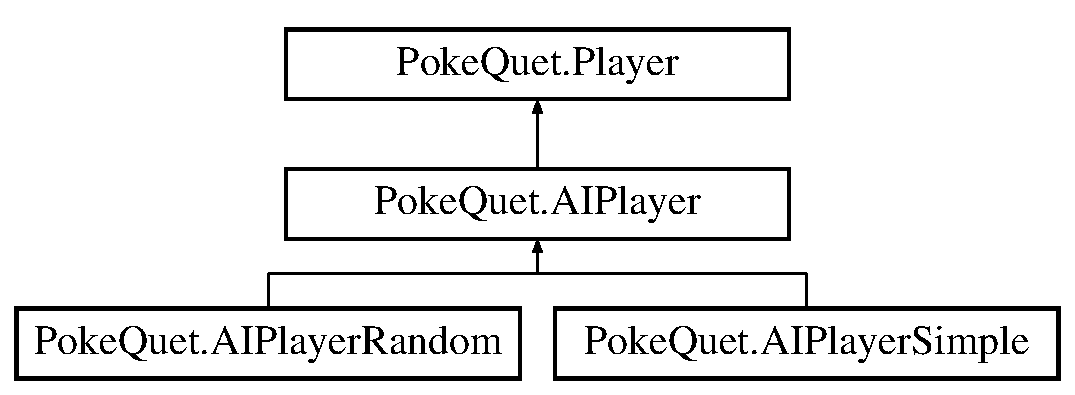
\includegraphics[height=3.000000cm]{class_poke_quet_1_1_player}
\end{center}
\end{figure}
\subsection*{Public Member Functions}
\begin{DoxyCompactItemize}
\item 
\mbox{\Hypertarget{class_poke_quet_1_1_player_ad78e2de62603112285cf59a609d5c705}\label{class_poke_quet_1_1_player_ad78e2de62603112285cf59a609d5c705}} 
{\bfseries Player} (string name)
\end{DoxyCompactItemize}
\subsection*{Static Public Attributes}
\begin{DoxyCompactItemize}
\item 
static readonly Random \mbox{\hyperlink{class_poke_quet_1_1_player_a0ea964b34febb9e63ed847d944ffcadf}{R\+NG}} = new Random()
\begin{DoxyCompactList}\small\item\em Ein Random Number Generator, Statisch um Zufälligkeit besser zu gewährleisten und ständige Neuerzeugung des Objekts vorzubeugen \end{DoxyCompactList}\end{DoxyCompactItemize}
\subsection*{Properties}
\begin{DoxyCompactItemize}
\item 
\mbox{\hyperlink{class_poke_quet_1_1_deck}{Deck}} \mbox{\hyperlink{class_poke_quet_1_1_player_af3e3987ecb9c2a43d233975e3cc414ff}{Deck}} = new \mbox{\hyperlink{class_poke_quet_1_1_deck}{Deck}}()\hspace{0.3cm}{\ttfamily  \mbox{[}get\mbox{]}}
\begin{DoxyCompactList}\small\item\em Das \mbox{\hyperlink{class_poke_quet_1_1_deck}{Deck}} des Spielers \end{DoxyCompactList}\item 
string \mbox{\hyperlink{class_poke_quet_1_1_player_a2ccd0df63845bdec5e75d80df2748ab5}{Name}}\hspace{0.3cm}{\ttfamily  \mbox{[}get, set\mbox{]}}
\begin{DoxyCompactList}\small\item\em Der Name des Spielers \end{DoxyCompactList}\end{DoxyCompactItemize}


\subsection{Member Data Documentation}
\mbox{\Hypertarget{class_poke_quet_1_1_player_a0ea964b34febb9e63ed847d944ffcadf}\label{class_poke_quet_1_1_player_a0ea964b34febb9e63ed847d944ffcadf}} 
\index{Poke\+Quet\+::\+Player@{Poke\+Quet\+::\+Player}!R\+NG@{R\+NG}}
\index{R\+NG@{R\+NG}!Poke\+Quet\+::\+Player@{Poke\+Quet\+::\+Player}}
\subsubsection{\texorpdfstring{R\+NG}{RNG}}
{\footnotesize\ttfamily readonly Random Poke\+Quet.\+Player.\+R\+NG = new Random()\hspace{0.3cm}{\ttfamily [static]}}



Ein Random Number Generator, Statisch um Zufälligkeit besser zu gewährleisten und ständige Neuerzeugung des Objekts vorzubeugen 



\subsection{Property Documentation}
\mbox{\Hypertarget{class_poke_quet_1_1_player_af3e3987ecb9c2a43d233975e3cc414ff}\label{class_poke_quet_1_1_player_af3e3987ecb9c2a43d233975e3cc414ff}} 
\index{Poke\+Quet\+::\+Player@{Poke\+Quet\+::\+Player}!Deck@{Deck}}
\index{Deck@{Deck}!Poke\+Quet\+::\+Player@{Poke\+Quet\+::\+Player}}
\subsubsection{\texorpdfstring{Deck}{Deck}}
{\footnotesize\ttfamily \mbox{\hyperlink{class_poke_quet_1_1_deck}{Deck}} Poke\+Quet.\+Player.\+Deck = new \mbox{\hyperlink{class_poke_quet_1_1_deck}{Deck}}()\hspace{0.3cm}{\ttfamily [get]}}



Das \mbox{\hyperlink{class_poke_quet_1_1_deck}{Deck}} des Spielers 

\mbox{\Hypertarget{class_poke_quet_1_1_player_a2ccd0df63845bdec5e75d80df2748ab5}\label{class_poke_quet_1_1_player_a2ccd0df63845bdec5e75d80df2748ab5}} 
\index{Poke\+Quet\+::\+Player@{Poke\+Quet\+::\+Player}!Name@{Name}}
\index{Name@{Name}!Poke\+Quet\+::\+Player@{Poke\+Quet\+::\+Player}}
\subsubsection{\texorpdfstring{Name}{Name}}
{\footnotesize\ttfamily string Poke\+Quet.\+Player.\+Name\hspace{0.3cm}{\ttfamily [get]}, {\ttfamily [set]}}



Der Name des Spielers 



The documentation for this class was generated from the following file\+:\begin{DoxyCompactItemize}
\item 
Player.\+cs\end{DoxyCompactItemize}

%--- End generated contents ---

% Index
\backmatter
\newpage
\phantomsection
\clearemptydoublepage
\addcontentsline{toc}{chapter}{Index}
\printindex

\end{document}
